\documentclass[11pt]{amsart}

\usepackage[T1]{fontenc}
\usepackage{lmodern}
\usepackage{microtype}
\usepackage{mathtools}
\usepackage{amssymb}
\usepackage{enumitem}
\usepackage{xcolor}
\usepackage{tikz}
\usepackage{hyperref}
\usepackage[nameinlink,noabbrev]{cleveref}
\usepackage{geometry}
\geometry{margin=1.08in}

\hypersetup{
  colorlinks=true,
  linkcolor=blue!45!black,
  citecolor=green!35!black,
  urlcolor=blue!55!black,
  pdfauthor={Mansehej Singh},
  pdftitle={Exact non-scattering homogeneous dielectrics from Schiffer counterexamples}
}

\newtheorem{theorem}{Theorem}[section]
\newtheorem{corollary}[theorem]{Corollary}
\newtheorem{proposition}[theorem]{Proposition}
\newtheorem{lemma}[theorem]{Lemma}
\newtheorem{remark}[theorem]{Remark}
\newtheorem{definition}[theorem]{Definition}

\newcommand{\D}{\mathbb D}
\newcommand{\R}{\mathbb R}
\newcommand{\C}{\mathbb C}
\newcommand{\Sone}{\mathbb S^1}
\newcommand{\norm}[1]{\left\lVert #1\right\rVert}
\newcommand{\abs}[1]{\left\lvert #1\right\rvert}
\newcommand{\dd}{\,\mathrm d}
\newcommand{\Rea}{\operatorname{Re}}

\title[Exact non-scattering dielectrics from Schiffer counterexamples]
{Exact non-scattering homogeneous dielectrics from Schiffer counterexamples}

\author{Mansehej Singh}
\address{Bristol, United Kingdom}
\date{19 August 2026}

\subjclass[2020]{Primary 35P25, 35R30; Secondary 65G20, 78A45, 30C35}
\keywords{non-scattering inclusion, Schiffer conjecture, Pompeiu problem,
transmission eigenvalue, Herglotz wave, computer-assisted proof}

\begin{document}

\begin{abstract}
We prove the existence of bounded, simply connected, noncircular homogeneous
isotropic dielectric inclusions that are exactly non-scattering for a
nonzero physical incident field in the two-dimensional scalar Maxwell
reduction.  The incident field is the explicit normalized Herglotz wave
\[
  v(x)=\sqrt{2\pi}\,J_0(\abs{x}),
  \qquad h(d)=\frac1{\sqrt{2\pi}},
\]
at exterior wavenumber one.  The construction starts from the
computer-assisted noncircular Schiffer counterexample of Colbrook and
Stepaniants.  We replace its constant boundary datum by a small-frequency
Bessel wave, prove that the regular Schiffer zero persists, and certify the
continuation uniformly for every $0<\tau\le10^{-13}$.  After dilation, the
resulting domain and constant relative permittivity are
\[
  \Omega_\tau=\sqrt\tau\,\phi_{p_\tau}(\D),
  \qquad q_\tau=\frac{p_{\tau,0}^2}{\tau}.
\]
An interior Helmholtz field matches both Cauchy traces of $v$ exactly, so the
radiating scattered field and its far-field pattern vanish identically.  As
a consequence, every prescribed contrast $Q\ge1.03\times10^{16}$ occurs for
some noncircular member of the family.
\end{abstract}

\maketitle

\section{Introduction}

Let $D\subset\R^2$ be a bounded dielectric inclusion with constant relative
permittivity $q>0$ and constant magnetic permeability.  In the
out-of-plane-electric scalar reduction of time-harmonic Maxwell equations,
an incident field $v$ at exterior wavenumber $k>0$ is physical when it is a
nonzero entire solution of
\begin{equation}\label{eq:incident}
  (\Delta+k^2)v=0\qquad\text{in }\R^2.
\end{equation}
Exact non-scattering requires an interior field $U$ satisfying
\begin{equation}\label{eq:interior}
  (\Delta+k^2q)U=0\qquad\text{in }D
\end{equation}
and the two trace identities
\begin{equation}\label{eq:traces}
  U=v,
  \qquad
  \partial_\nu U=\partial_\nu v
  \qquad\text{on }\partial D.
\end{equation}
Then the exterior total field may equal $v$ itself, so the scattered field is
the zero radiating solution.  This is stronger than the mere existence of a
transmission eigenvalue: the incident component must extend to an entire
physical Helmholtz solution, and in the present theorem it is an
$L^2$-Herglotz wave.  The distinction is emphasized in
\cite{HovsepyanVogelius2025,CakoniVogelius2026}.

Two lines of prior work frame this question.  First, geometric
obstructions: domains with corners scatter every incident wave
\cite{BlastenPaivarintaSylvester2014,PaivarintaSaloVesalainen2017,
ElschnerHu2015}, and non-scattering forces strong boundary regularity
\cite{SaloShahgholian2021,CakoniVogelius2023,CakoniVogeliusXiao2023}, so
any example must have smooth, indeed essentially real-analytic, boundary.
Second, spectral necessity: non-scattering requires an interior
transmission eigenpair \cite{Kirsch1986,ColtonMonk1988,
CakoniColtonHaddar2016}, but a transmission eigenpair alone does not supply
a physical incident field, and for broad families of perturbed discs the
nonscattering wave numbers of physical incident waves are at most finite
\cite{VogeliusXiao2021,HovsepyanVogelius2025}.  Radial homogeneous
inclusions are the classical exception; whether any noncircular homogeneous
inclusion admits an exactly non-scattering physical incident wave has
remained open \cite{CakoniVogelius2026}.

A neighboring overdetermined problem is Schiffer's conjecture, which is
closely tied to the Pompeiu problem
\cite{Pompeiu1929,BrownSchreiberTaylor1973,Williams1976,Berenstein1980}.
It asks whether a bounded domain admitting a nonconstant solution of
\begin{equation}\label{eq:schiffer-intro}
  (\Delta+\lambda)u=0\quad\text{in }D,
  \qquad
  u=1,
  \quad
  \partial_\nu u=0
  \quad\text{on }\partial D
\end{equation}
must be a disc.  Colbrook and Stepaniants recently constructed a
computer-assisted noncircular counterexample with real-analytic boundary,
and Cao-Labora and de Dios Pont independently produced infinitely many
bifurcating counterexamples
\cite{ColbrookStepaniants2026,CaoLaboraDeDiosPont2026}.  These results do not
immediately solve the scattering problem: at positive frequency the constant
function $1$ does not satisfy the exterior Helmholtz equation.

The central observation of this paper is that the Schiffer datum can be
replaced by a genuine radial Helmholtz wave.  More precisely, a regular
Schiffer zero persists when the constant boundary datum is deformed to
\[
  J_0(\sqrt\tau\,\abs{x})=1-\frac\tau4\abs{x}^2+O(\tau^2).
\]
The resulting transmission pair has exterior squared wavenumber $\tau$ and
interior squared wavenumber close to the Schiffer eigenvalue.  A final
dilation fixes the exterior wavenumber at $k=1$.  This answers the
constant-index, noncircular, physical-incident-field existence question
affirmatively in the two-dimensional scalar model.  Thus the construction is a
subwavelength, high-contrast resonance: the physical diameter shrinks like
$\sqrt\tau$, while the interior optical size remains finite.

\subsection{Main result}

Let
\begin{equation}\label{eq:herglotz}
  h(d)=\frac1{\sqrt{2\pi}},
  \qquad
  v(x)=\int_{\Sone}e^{ix\cdot d}h(d)\dd s(d)
      =\sqrt{2\pi}\,J_0(\abs{x}).
\end{equation}
Then $h\in L^2(\Sone)$, $\norm{h}_{L^2}=1$, and $(\Delta+1)v=0$ in
$\R^2$.

\begin{theorem}[Exact non-scattering family]\label{thm:main}
For every $0<\tau\le10^{-13}$ there exist a bounded simply connected domain
$\Omega_\tau\subset\R^2$, a constant $q_\tau>0$, and an interior field
$U_\tau$ such that:
\begin{enumerate}[label=\textup{(\roman*)},leftmargin=2.2em]
  \item $\partial\Omega_\tau$ is a real-analytic Jordan curve and
  $\Omega_\tau$ is not a disc;
  \item $q_\tau\ne1$;
  \item
  \[
    (\Delta+q_\tau)U_\tau=0\quad\text{in }\Omega_\tau;
  \]
  \item $U_\tau=v$ and
  $\partial_\nu U_\tau=\partial_\nu v$ on $\partial\Omega_\tau$.
\end{enumerate}
Consequently the radiating scattered field and the far-field pattern vanish
identically for the normalized Herglotz incident wave \eqref{eq:herglotz} at
exterior wavenumber $k=1$.
\end{theorem}

The construction is exact, not a finite multipole cancellation.  For each
$\tau$, a contraction theorem selects a unique infinite coefficient pair
$(\gamma_\tau,p_\tau)$ in a fixed certified Banach ball.  If
\begin{equation}\label{eq:phi}
  \phi_p(z)=z+\sum_{j\ge1}
  \frac{p_j}{p_0(10j+1)}z^{10j+1},
\end{equation}
then
\begin{equation}\label{eq:Omegaq}
  \Omega_\tau=\sqrt\tau\,\phi_{p_\tau}(\D),
  \qquad
  q_\tau=\frac{p_{\tau,0}^2}{\tau}.
\end{equation}

\begin{figure}[t]
  \centering
  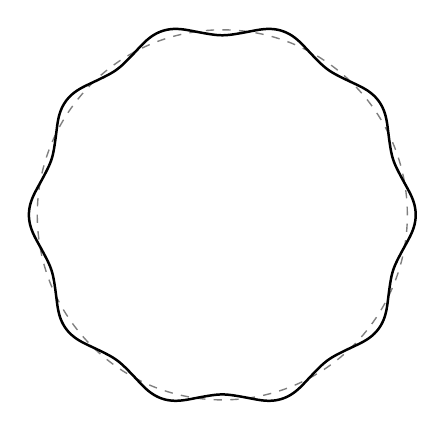
\begin{tikzpicture}[baseline=(current bounding box.center), scale=2.35]
  \draw[dashed, gray, line width=0.5pt] (0,0) circle (1);
  \draw[line width=0.9pt] plot coordinates {(1.04513,0.00000) (1.04501,0.00719) (1.04465,0.01436) (1.04406,0.02148) (1.04324,0.02854) (1.04220,0.03551) (1.04096,0.04238) (1.03953,0.04912) (1.03793,0.05573) (1.03617,0.06219) (1.03427,0.06851) (1.03225,0.07466) (1.03013,0.08065) (1.02792,0.08647) (1.02564,0.09213) (1.02331,0.09763) (1.02094,0.10297) (1.01855,0.10816) (1.01613,0.11321) (1.01372,0.11811) (1.01130,0.12289) (1.00890,0.12754) (1.00651,0.13208) (1.00415,0.13651) (1.00182,0.14084) (0.99951,0.14508) (0.99723,0.14923) (0.99499,0.15331) (0.99278,0.15731) (0.99060,0.16124) (0.98846,0.16512) (0.98635,0.16893) (0.98428,0.17270) (0.98224,0.17641) (0.98022,0.18008) (0.97824,0.18371) (0.97629,0.18729) (0.97436,0.19084) (0.97246,0.19435) (0.97058,0.19783) (0.96874,0.20128) (0.96691,0.20469) (0.96511,0.20807) (0.96333,0.21143) (0.96157,0.21475) (0.95984,0.21804) (0.95813,0.22131) (0.95644,0.22455) (0.95478,0.22777) (0.95314,0.23096) (0.95152,0.23412) (0.94993,0.23726) (0.94836,0.24038) (0.94681,0.24348) (0.94530,0.24655) (0.94381,0.24961) (0.94234,0.25265) (0.94091,0.25567) (0.93950,0.25867) (0.93813,0.26166) (0.93678,0.26463) (0.93546,0.26760) (0.93417,0.27055) (0.93292,0.27349) (0.93169,0.27643) (0.93050,0.27936) (0.92934,0.28229) (0.92821,0.28522) (0.92711,0.28815) (0.92604,0.29108) (0.92500,0.29402) (0.92400,0.29696) (0.92302,0.29991) (0.92208,0.30287) (0.92116,0.30584) (0.92028,0.30882) (0.91942,0.31182) (0.91858,0.31484) (0.91778,0.31787) (0.91700,0.32092) (0.91624,0.32400) (0.91550,0.32709) (0.91479,0.33021) (0.91409,0.33336) (0.91342,0.33653) (0.91276,0.33973) (0.91212,0.34296) (0.91149,0.34621) (0.91087,0.34950) (0.91027,0.35282) (0.90968,0.35617) (0.90910,0.35955) (0.90853,0.36296) (0.90797,0.36640) (0.90741,0.36988) (0.90686,0.37339) (0.90631,0.37694) (0.90577,0.38052) (0.90523,0.38413) (0.90469,0.38778) (0.90416,0.39146) (0.90362,0.39518) (0.90309,0.39894) (0.90256,0.40274) (0.90203,0.40657) (0.90150,0.41045) (0.90097,0.41436) (0.90045,0.41832) (0.89992,0.42232) (0.89939,0.42637) (0.89887,0.43047) (0.89834,0.43462) (0.89781,0.43883) (0.89727,0.44309) (0.89674,0.44742) (0.89619,0.45181) (0.89564,0.45628) (0.89507,0.46081) (0.89449,0.46543) (0.89389,0.47012) (0.89327,0.47491) (0.89262,0.47979) (0.89192,0.48476) (0.89119,0.48983) (0.89039,0.49501) (0.88954,0.50029) (0.88861,0.50568) (0.88760,0.51118) (0.88648,0.51679) (0.88526,0.52251) (0.88392,0.52832) (0.88243,0.53424) (0.88079,0.54025) (0.87899,0.54634) (0.87701,0.55251) (0.87483,0.55873) (0.87246,0.56499) (0.86987,0.57128) (0.86706,0.57758) (0.86403,0.58386) (0.86078,0.59011) (0.85729,0.59630) (0.85358,0.60241) (0.84966,0.60842) (0.84553,0.61431) (0.84121,0.62006) (0.83670,0.62565) (0.83203,0.63106) (0.82722,0.63629) (0.82229,0.64132) (0.81725,0.64615) (0.81213,0.65076) (0.80694,0.65517) (0.80172,0.65936) (0.79648,0.66335) (0.79123,0.66714) (0.78599,0.67074) (0.78078,0.67415) (0.77561,0.67739) (0.77049,0.68047) (0.76543,0.68340) (0.76044,0.68619) (0.75553,0.68885) (0.75069,0.69140) (0.74593,0.69385) (0.74125,0.69620) (0.73665,0.69847) (0.73214,0.70067) (0.72770,0.70280) (0.72334,0.70487) (0.71906,0.70689) (0.71485,0.70887) (0.71071,0.71081) (0.70664,0.71271) (0.70263,0.71459) (0.69868,0.71644) (0.69479,0.71826) (0.69095,0.72006) (0.68717,0.72185) (0.68343,0.72362) (0.67974,0.72537) (0.67610,0.72711) (0.67250,0.72883) (0.66894,0.73054) (0.66542,0.73224) (0.66193,0.73393) (0.65849,0.73561) (0.65508,0.73728) (0.65170,0.73893) (0.64836,0.74058) (0.64506,0.74222) (0.64179,0.74385) (0.63855,0.74547) (0.63535,0.74709) (0.63218,0.74870) (0.62905,0.75030) (0.62594,0.75190) (0.62288,0.75350) (0.61984,0.75510) (0.61684,0.75669) (0.61387,0.75829) (0.61093,0.75989) (0.60803,0.76149) (0.60516,0.76310) (0.60232,0.76472) (0.59951,0.76634) (0.59674,0.76797) (0.59399,0.76962) (0.59127,0.77127) (0.58858,0.77294) (0.58592,0.77463) (0.58329,0.77634) (0.58067,0.77806) (0.57809,0.77980) (0.57552,0.78157) (0.57298,0.78336) (0.57046,0.78517) (0.56796,0.78701) (0.56547,0.78888) (0.56300,0.79077) (0.56054,0.79269) (0.55809,0.79464) (0.55566,0.79662) (0.55323,0.79863) (0.55081,0.80067) (0.54839,0.80274) (0.54598,0.80485) (0.54357,0.80698) (0.54116,0.80915) (0.53875,0.81135) (0.53633,0.81359) (0.53391,0.81585) (0.53148,0.81815) (0.52905,0.82048) (0.52660,0.82284) (0.52414,0.82524) (0.52168,0.82766) (0.51920,0.83011) (0.51670,0.83260) (0.51419,0.83512) (0.51166,0.83766) (0.50912,0.84024) (0.50656,0.84285) (0.50398,0.84548) (0.50138,0.84815) (0.49876,0.85085) (0.49612,0.85357) (0.49346,0.85633) (0.49078,0.85912) (0.48808,0.86195) (0.48535,0.86480) (0.48260,0.86770) (0.47982,0.87063) (0.47701,0.87359) (0.47417,0.87660) (0.47131,0.87965) (0.46840,0.88274) (0.46547,0.88588) (0.46249,0.88906) (0.45947,0.89229) (0.45640,0.89558) (0.45327,0.89892) (0.45009,0.90231) (0.44684,0.90576) (0.44353,0.90926) (0.44013,0.91282) (0.43665,0.91644) (0.43307,0.92011) (0.42939,0.92383) (0.42559,0.92760) (0.42167,0.93142) (0.41762,0.93527) (0.41342,0.93915) (0.40907,0.94306) (0.40456,0.94698) (0.39988,0.95089) (0.39503,0.95479) (0.38999,0.95866) (0.38476,0.96248) (0.37934,0.96624) (0.37374,0.96991) (0.36795,0.97347) (0.36198,0.97692) (0.35583,0.98022) (0.34952,0.98336) (0.34307,0.98632) (0.33647,0.98909) (0.32977,0.99164) (0.32296,0.99398) (0.31609,0.99609) (0.30916,0.99796) (0.30220,0.99960) (0.29523,1.00100) (0.28828,1.00217) (0.28137,1.00311) (0.27452,1.00383) (0.26773,1.00435) (0.26104,1.00467) (0.25445,1.00482) (0.24798,1.00480) (0.24163,1.00463) (0.23541,1.00433) (0.22932,1.00391) (0.22337,1.00340) (0.21756,1.00279) (0.21188,1.00212) (0.20634,1.00138) (0.20092,1.00060) (0.19563,0.99978) (0.19047,0.99893) (0.18541,0.99807) (0.18047,0.99719) (0.17563,0.99631) (0.17089,0.99542) (0.16623,0.99454) (0.16166,0.99367) (0.15718,0.99280) (0.15276,0.99195) (0.14842,0.99111) (0.14413,0.99028) (0.13991,0.98947) (0.13575,0.98868) (0.13164,0.98790) (0.12758,0.98713) (0.12356,0.98638) (0.11959,0.98564) (0.11566,0.98492) (0.11178,0.98421) (0.10793,0.98352) (0.10412,0.98284) (0.10035,0.98217) (0.09661,0.98151) (0.09290,0.98087) (0.08923,0.98024) (0.08560,0.97962) (0.08199,0.97902) (0.07842,0.97843) (0.07488,0.97786) (0.07137,0.97730) (0.06789,0.97675) (0.06444,0.97622) (0.06102,0.97571) (0.05763,0.97522) (0.05426,0.97475) (0.05092,0.97430) (0.04760,0.97386) (0.04431,0.97345) (0.04105,0.97307) (0.03780,0.97270) (0.03457,0.97237) (0.03137,0.97206) (0.02818,0.97177) (0.02501,0.97151) (0.02185,0.97128) (0.01870,0.97109) (0.01557,0.97092) (0.01244,0.97078) (0.00933,0.97067) (0.00621,0.97059) (0.00311,0.97054) (0.00000,0.97053) (-0.00311,0.97054) (-0.00621,0.97059) (-0.00933,0.97067) (-0.01244,0.97078) (-0.01557,0.97092) (-0.01870,0.97109) (-0.02185,0.97128) (-0.02501,0.97151) (-0.02818,0.97177) (-0.03137,0.97206) (-0.03457,0.97237) (-0.03780,0.97270) (-0.04105,0.97307) (-0.04431,0.97345) (-0.04760,0.97386) (-0.05092,0.97430) (-0.05426,0.97475) (-0.05763,0.97522) (-0.06102,0.97571) (-0.06444,0.97622) (-0.06789,0.97675) (-0.07137,0.97730) (-0.07488,0.97786) (-0.07842,0.97843) (-0.08199,0.97902) (-0.08560,0.97962) (-0.08923,0.98024) (-0.09290,0.98087) (-0.09661,0.98151) (-0.10035,0.98217) (-0.10412,0.98284) (-0.10793,0.98352) (-0.11178,0.98421) (-0.11566,0.98492) (-0.11959,0.98564) (-0.12356,0.98638) (-0.12758,0.98713) (-0.13164,0.98790) (-0.13575,0.98868) (-0.13991,0.98947) (-0.14413,0.99028) (-0.14842,0.99111) (-0.15276,0.99195) (-0.15718,0.99280) (-0.16166,0.99367) (-0.16623,0.99454) (-0.17089,0.99542) (-0.17563,0.99631) (-0.18047,0.99719) (-0.18541,0.99807) (-0.19047,0.99893) (-0.19563,0.99978) (-0.20092,1.00060) (-0.20634,1.00138) (-0.21188,1.00212) (-0.21756,1.00279) (-0.22337,1.00340) (-0.22932,1.00391) (-0.23541,1.00433) (-0.24163,1.00463) (-0.24798,1.00480) (-0.25445,1.00482) (-0.26104,1.00467) (-0.26773,1.00435) (-0.27452,1.00383) (-0.28137,1.00311) (-0.28828,1.00217) (-0.29523,1.00100) (-0.30220,0.99960) (-0.30916,0.99796) (-0.31609,0.99609) (-0.32296,0.99398) (-0.32977,0.99164) (-0.33647,0.98909) (-0.34307,0.98632) (-0.34952,0.98336) (-0.35583,0.98022) (-0.36198,0.97692) (-0.36795,0.97347) (-0.37374,0.96991) (-0.37934,0.96624) (-0.38476,0.96248) (-0.38999,0.95866) (-0.39503,0.95479) (-0.39988,0.95089) (-0.40456,0.94698) (-0.40907,0.94306) (-0.41342,0.93915) (-0.41762,0.93527) (-0.42167,0.93142) (-0.42559,0.92760) (-0.42939,0.92383) (-0.43307,0.92011) (-0.43665,0.91644) (-0.44013,0.91282) (-0.44353,0.90926) (-0.44684,0.90576) (-0.45009,0.90231) (-0.45327,0.89892) (-0.45640,0.89558) (-0.45947,0.89229) (-0.46249,0.88906) (-0.46547,0.88588) (-0.46840,0.88274) (-0.47131,0.87965) (-0.47417,0.87660) (-0.47701,0.87359) (-0.47982,0.87063) (-0.48260,0.86770) (-0.48535,0.86480) (-0.48808,0.86195) (-0.49078,0.85912) (-0.49346,0.85633) (-0.49612,0.85357) (-0.49876,0.85085) (-0.50138,0.84815) (-0.50398,0.84548) (-0.50656,0.84285) (-0.50912,0.84024) (-0.51166,0.83766) (-0.51419,0.83512) (-0.51670,0.83260) (-0.51920,0.83011) (-0.52168,0.82766) (-0.52414,0.82524) (-0.52660,0.82284) (-0.52905,0.82048) (-0.53148,0.81815) (-0.53391,0.81585) (-0.53633,0.81359) (-0.53875,0.81135) (-0.54116,0.80915) (-0.54357,0.80698) (-0.54598,0.80485) (-0.54839,0.80274) (-0.55081,0.80067) (-0.55323,0.79863) (-0.55566,0.79662) (-0.55809,0.79464) (-0.56054,0.79269) (-0.56300,0.79077) (-0.56547,0.78888) (-0.56796,0.78701) (-0.57046,0.78517) (-0.57298,0.78336) (-0.57552,0.78157) (-0.57809,0.77980) (-0.58067,0.77806) (-0.58329,0.77634) (-0.58592,0.77463) (-0.58858,0.77294) (-0.59127,0.77127) (-0.59399,0.76962) (-0.59674,0.76797) (-0.59951,0.76634) (-0.60232,0.76472) (-0.60516,0.76310) (-0.60803,0.76149) (-0.61093,0.75989) (-0.61387,0.75829) (-0.61684,0.75669) (-0.61984,0.75510) (-0.62288,0.75350) (-0.62594,0.75190) (-0.62905,0.75030) (-0.63218,0.74870) (-0.63535,0.74709) (-0.63855,0.74547) (-0.64179,0.74385) (-0.64506,0.74222) (-0.64836,0.74058) (-0.65170,0.73893) (-0.65508,0.73728) (-0.65849,0.73561) (-0.66193,0.73393) (-0.66542,0.73224) (-0.66894,0.73054) (-0.67250,0.72883) (-0.67610,0.72711) (-0.67974,0.72537) (-0.68343,0.72362) (-0.68717,0.72185) (-0.69095,0.72006) (-0.69479,0.71826) (-0.69868,0.71644) (-0.70263,0.71459) (-0.70664,0.71271) (-0.71071,0.71081) (-0.71485,0.70887) (-0.71906,0.70689) (-0.72334,0.70487) (-0.72770,0.70280) (-0.73214,0.70067) (-0.73665,0.69847) (-0.74125,0.69620) (-0.74593,0.69385) (-0.75069,0.69140) (-0.75553,0.68885) (-0.76044,0.68619) (-0.76543,0.68340) (-0.77049,0.68047) (-0.77561,0.67739) (-0.78078,0.67415) (-0.78599,0.67074) (-0.79123,0.66714) (-0.79648,0.66335) (-0.80172,0.65936) (-0.80694,0.65517) (-0.81213,0.65076) (-0.81725,0.64615) (-0.82229,0.64132) (-0.82722,0.63629) (-0.83203,0.63106) (-0.83670,0.62565) (-0.84121,0.62006) (-0.84553,0.61431) (-0.84966,0.60842) (-0.85358,0.60241) (-0.85729,0.59630) (-0.86078,0.59011) (-0.86403,0.58386) (-0.86706,0.57758) (-0.86987,0.57128) (-0.87246,0.56499) (-0.87483,0.55873) (-0.87701,0.55251) (-0.87899,0.54634) (-0.88079,0.54025) (-0.88243,0.53424) (-0.88392,0.52832) (-0.88526,0.52251) (-0.88648,0.51679) (-0.88760,0.51118) (-0.88861,0.50568) (-0.88954,0.50029) (-0.89039,0.49501) (-0.89119,0.48983) (-0.89192,0.48476) (-0.89262,0.47979) (-0.89327,0.47491) (-0.89389,0.47012) (-0.89449,0.46543) (-0.89507,0.46081) (-0.89564,0.45628) (-0.89619,0.45181) (-0.89674,0.44742) (-0.89727,0.44309) (-0.89781,0.43883) (-0.89834,0.43462) (-0.89887,0.43047) (-0.89939,0.42637) (-0.89992,0.42232) (-0.90045,0.41832) (-0.90097,0.41436) (-0.90150,0.41045) (-0.90203,0.40657) (-0.90256,0.40274) (-0.90309,0.39894) (-0.90362,0.39518) (-0.90416,0.39146) (-0.90469,0.38778) (-0.90523,0.38413) (-0.90577,0.38052) (-0.90631,0.37694) (-0.90686,0.37339) (-0.90741,0.36988) (-0.90797,0.36640) (-0.90853,0.36296) (-0.90910,0.35955) (-0.90968,0.35617) (-0.91027,0.35282) (-0.91087,0.34950) (-0.91149,0.34621) (-0.91212,0.34296) (-0.91276,0.33973) (-0.91342,0.33653) (-0.91409,0.33336) (-0.91479,0.33021) (-0.91550,0.32709) (-0.91624,0.32400) (-0.91700,0.32092) (-0.91778,0.31787) (-0.91858,0.31484) (-0.91942,0.31182) (-0.92028,0.30882) (-0.92116,0.30584) (-0.92208,0.30287) (-0.92302,0.29991) (-0.92400,0.29696) (-0.92500,0.29402) (-0.92604,0.29108) (-0.92711,0.28815) (-0.92821,0.28522) (-0.92934,0.28229) (-0.93050,0.27936) (-0.93169,0.27643) (-0.93292,0.27349) (-0.93417,0.27055) (-0.93546,0.26760) (-0.93678,0.26463) (-0.93813,0.26166) (-0.93950,0.25867) (-0.94091,0.25567) (-0.94234,0.25265) (-0.94381,0.24961) (-0.94530,0.24655) (-0.94681,0.24348) (-0.94836,0.24038) (-0.94993,0.23726) (-0.95152,0.23412) (-0.95314,0.23096) (-0.95478,0.22777) (-0.95644,0.22455) (-0.95813,0.22131) (-0.95984,0.21804) (-0.96157,0.21475) (-0.96333,0.21143) (-0.96511,0.20807) (-0.96691,0.20469) (-0.96874,0.20128) (-0.97058,0.19783) (-0.97246,0.19435) (-0.97436,0.19084) (-0.97629,0.18729) (-0.97824,0.18371) (-0.98022,0.18008) (-0.98224,0.17641) (-0.98428,0.17270) (-0.98635,0.16893) (-0.98846,0.16512) (-0.99060,0.16124) (-0.99278,0.15731) (-0.99499,0.15331) (-0.99723,0.14923) (-0.99951,0.14508) (-1.00182,0.14084) (-1.00415,0.13651) (-1.00651,0.13208) (-1.00890,0.12754) (-1.01130,0.12289) (-1.01372,0.11811) (-1.01613,0.11321) (-1.01855,0.10816) (-1.02094,0.10297) (-1.02331,0.09763) (-1.02564,0.09213) (-1.02792,0.08647) (-1.03013,0.08065) (-1.03225,0.07466) (-1.03427,0.06851) (-1.03617,0.06219) (-1.03793,0.05573) (-1.03953,0.04912) (-1.04096,0.04238) (-1.04220,0.03551) (-1.04324,0.02854) (-1.04406,0.02148) (-1.04465,0.01436) (-1.04501,0.00719) (-1.04513,0.00000) (-1.04501,-0.00719) (-1.04465,-0.01436) (-1.04406,-0.02148) (-1.04324,-0.02854) (-1.04220,-0.03551) (-1.04096,-0.04238) (-1.03953,-0.04912) (-1.03793,-0.05573) (-1.03617,-0.06219) (-1.03427,-0.06851) (-1.03225,-0.07466) (-1.03013,-0.08065) (-1.02792,-0.08647) (-1.02564,-0.09213) (-1.02331,-0.09763) (-1.02094,-0.10297) (-1.01855,-0.10816) (-1.01613,-0.11321) (-1.01372,-0.11811) (-1.01130,-0.12289) (-1.00890,-0.12754) (-1.00651,-0.13208) (-1.00415,-0.13651) (-1.00182,-0.14084) (-0.99951,-0.14508) (-0.99723,-0.14923) (-0.99499,-0.15331) (-0.99278,-0.15731) (-0.99060,-0.16124) (-0.98846,-0.16512) (-0.98635,-0.16893) (-0.98428,-0.17270) (-0.98224,-0.17641) (-0.98022,-0.18008) (-0.97824,-0.18371) (-0.97629,-0.18729) (-0.97436,-0.19084) (-0.97246,-0.19435) (-0.97058,-0.19783) (-0.96874,-0.20128) (-0.96691,-0.20469) (-0.96511,-0.20807) (-0.96333,-0.21143) (-0.96157,-0.21475) (-0.95984,-0.21804) (-0.95813,-0.22131) (-0.95644,-0.22455) (-0.95478,-0.22777) (-0.95314,-0.23096) (-0.95152,-0.23412) (-0.94993,-0.23726) (-0.94836,-0.24038) (-0.94681,-0.24348) (-0.94530,-0.24655) (-0.94381,-0.24961) (-0.94234,-0.25265) (-0.94091,-0.25567) (-0.93950,-0.25867) (-0.93813,-0.26166) (-0.93678,-0.26463) (-0.93546,-0.26760) (-0.93417,-0.27055) (-0.93292,-0.27349) (-0.93169,-0.27643) (-0.93050,-0.27936) (-0.92934,-0.28229) (-0.92821,-0.28522) (-0.92711,-0.28815) (-0.92604,-0.29108) (-0.92500,-0.29402) (-0.92400,-0.29696) (-0.92302,-0.29991) (-0.92208,-0.30287) (-0.92116,-0.30584) (-0.92028,-0.30882) (-0.91942,-0.31182) (-0.91858,-0.31484) (-0.91778,-0.31787) (-0.91700,-0.32092) (-0.91624,-0.32400) (-0.91550,-0.32709) (-0.91479,-0.33021) (-0.91409,-0.33336) (-0.91342,-0.33653) (-0.91276,-0.33973) (-0.91212,-0.34296) (-0.91149,-0.34621) (-0.91087,-0.34950) (-0.91027,-0.35282) (-0.90968,-0.35617) (-0.90910,-0.35955) (-0.90853,-0.36296) (-0.90797,-0.36640) (-0.90741,-0.36988) (-0.90686,-0.37339) (-0.90631,-0.37694) (-0.90577,-0.38052) (-0.90523,-0.38413) (-0.90469,-0.38778) (-0.90416,-0.39146) (-0.90362,-0.39518) (-0.90309,-0.39894) (-0.90256,-0.40274) (-0.90203,-0.40657) (-0.90150,-0.41045) (-0.90097,-0.41436) (-0.90045,-0.41832) (-0.89992,-0.42232) (-0.89939,-0.42637) (-0.89887,-0.43047) (-0.89834,-0.43462) (-0.89781,-0.43883) (-0.89727,-0.44309) (-0.89674,-0.44742) (-0.89619,-0.45181) (-0.89564,-0.45628) (-0.89507,-0.46081) (-0.89449,-0.46543) (-0.89389,-0.47012) (-0.89327,-0.47491) (-0.89262,-0.47979) (-0.89192,-0.48476) (-0.89119,-0.48983) (-0.89039,-0.49501) (-0.88954,-0.50029) (-0.88861,-0.50568) (-0.88760,-0.51118) (-0.88648,-0.51679) (-0.88526,-0.52251) (-0.88392,-0.52832) (-0.88243,-0.53424) (-0.88079,-0.54025) (-0.87899,-0.54634) (-0.87701,-0.55251) (-0.87483,-0.55873) (-0.87246,-0.56499) (-0.86987,-0.57128) (-0.86706,-0.57758) (-0.86403,-0.58386) (-0.86078,-0.59011) (-0.85729,-0.59630) (-0.85358,-0.60241) (-0.84966,-0.60842) (-0.84553,-0.61431) (-0.84121,-0.62006) (-0.83670,-0.62565) (-0.83203,-0.63106) (-0.82722,-0.63629) (-0.82229,-0.64132) (-0.81725,-0.64615) (-0.81213,-0.65076) (-0.80694,-0.65517) (-0.80172,-0.65936) (-0.79648,-0.66335) (-0.79123,-0.66714) (-0.78599,-0.67074) (-0.78078,-0.67415) (-0.77561,-0.67739) (-0.77049,-0.68047) (-0.76543,-0.68340) (-0.76044,-0.68619) (-0.75553,-0.68885) (-0.75069,-0.69140) (-0.74593,-0.69385) (-0.74125,-0.69620) (-0.73665,-0.69847) (-0.73214,-0.70067) (-0.72770,-0.70280) (-0.72334,-0.70487) (-0.71906,-0.70689) (-0.71485,-0.70887) (-0.71071,-0.71081) (-0.70664,-0.71271) (-0.70263,-0.71459) (-0.69868,-0.71644) (-0.69479,-0.71826) (-0.69095,-0.72006) (-0.68717,-0.72185) (-0.68343,-0.72362) (-0.67974,-0.72537) (-0.67610,-0.72711) (-0.67250,-0.72883) (-0.66894,-0.73054) (-0.66542,-0.73224) (-0.66193,-0.73393) (-0.65849,-0.73561) (-0.65508,-0.73728) (-0.65170,-0.73893) (-0.64836,-0.74058) (-0.64506,-0.74222) (-0.64179,-0.74385) (-0.63855,-0.74547) (-0.63535,-0.74709) (-0.63218,-0.74870) (-0.62905,-0.75030) (-0.62594,-0.75190) (-0.62288,-0.75350) (-0.61984,-0.75510) (-0.61684,-0.75669) (-0.61387,-0.75829) (-0.61093,-0.75989) (-0.60803,-0.76149) (-0.60516,-0.76310) (-0.60232,-0.76472) (-0.59951,-0.76634) (-0.59674,-0.76797) (-0.59399,-0.76962) (-0.59127,-0.77127) (-0.58858,-0.77294) (-0.58592,-0.77463) (-0.58329,-0.77634) (-0.58067,-0.77806) (-0.57809,-0.77980) (-0.57552,-0.78157) (-0.57298,-0.78336) (-0.57046,-0.78517) (-0.56796,-0.78701) (-0.56547,-0.78888) (-0.56300,-0.79077) (-0.56054,-0.79269) (-0.55809,-0.79464) (-0.55566,-0.79662) (-0.55323,-0.79863) (-0.55081,-0.80067) (-0.54839,-0.80274) (-0.54598,-0.80485) (-0.54357,-0.80698) (-0.54116,-0.80915) (-0.53875,-0.81135) (-0.53633,-0.81359) (-0.53391,-0.81585) (-0.53148,-0.81815) (-0.52905,-0.82048) (-0.52660,-0.82284) (-0.52414,-0.82524) (-0.52168,-0.82766) (-0.51920,-0.83011) (-0.51670,-0.83260) (-0.51419,-0.83512) (-0.51166,-0.83766) (-0.50912,-0.84024) (-0.50656,-0.84285) (-0.50398,-0.84548) (-0.50138,-0.84815) (-0.49876,-0.85085) (-0.49612,-0.85357) (-0.49346,-0.85633) (-0.49078,-0.85912) (-0.48808,-0.86195) (-0.48535,-0.86480) (-0.48260,-0.86770) (-0.47982,-0.87063) (-0.47701,-0.87359) (-0.47417,-0.87660) (-0.47131,-0.87965) (-0.46840,-0.88274) (-0.46547,-0.88588) (-0.46249,-0.88906) (-0.45947,-0.89229) (-0.45640,-0.89558) (-0.45327,-0.89892) (-0.45009,-0.90231) (-0.44684,-0.90576) (-0.44353,-0.90926) (-0.44013,-0.91282) (-0.43665,-0.91644) (-0.43307,-0.92011) (-0.42939,-0.92383) (-0.42559,-0.92760) (-0.42167,-0.93142) (-0.41762,-0.93527) (-0.41342,-0.93915) (-0.40907,-0.94306) (-0.40456,-0.94698) (-0.39988,-0.95089) (-0.39503,-0.95479) (-0.38999,-0.95866) (-0.38476,-0.96248) (-0.37934,-0.96624) (-0.37374,-0.96991) (-0.36795,-0.97347) (-0.36198,-0.97692) (-0.35583,-0.98022) (-0.34952,-0.98336) (-0.34307,-0.98632) (-0.33647,-0.98909) (-0.32977,-0.99164) (-0.32296,-0.99398) (-0.31609,-0.99609) (-0.30916,-0.99796) (-0.30220,-0.99960) (-0.29523,-1.00100) (-0.28828,-1.00217) (-0.28137,-1.00311) (-0.27452,-1.00383) (-0.26773,-1.00435) (-0.26104,-1.00467) (-0.25445,-1.00482) (-0.24798,-1.00480) (-0.24163,-1.00463) (-0.23541,-1.00433) (-0.22932,-1.00391) (-0.22337,-1.00340) (-0.21756,-1.00279) (-0.21188,-1.00212) (-0.20634,-1.00138) (-0.20092,-1.00060) (-0.19563,-0.99978) (-0.19047,-0.99893) (-0.18541,-0.99807) (-0.18047,-0.99719) (-0.17563,-0.99631) (-0.17089,-0.99542) (-0.16623,-0.99454) (-0.16166,-0.99367) (-0.15718,-0.99280) (-0.15276,-0.99195) (-0.14842,-0.99111) (-0.14413,-0.99028) (-0.13991,-0.98947) (-0.13575,-0.98868) (-0.13164,-0.98790) (-0.12758,-0.98713) (-0.12356,-0.98638) (-0.11959,-0.98564) (-0.11566,-0.98492) (-0.11178,-0.98421) (-0.10793,-0.98352) (-0.10412,-0.98284) (-0.10035,-0.98217) (-0.09661,-0.98151) (-0.09290,-0.98087) (-0.08923,-0.98024) (-0.08560,-0.97962) (-0.08199,-0.97902) (-0.07842,-0.97843) (-0.07488,-0.97786) (-0.07137,-0.97730) (-0.06789,-0.97675) (-0.06444,-0.97622) (-0.06102,-0.97571) (-0.05763,-0.97522) (-0.05426,-0.97475) (-0.05092,-0.97430) (-0.04760,-0.97386) (-0.04431,-0.97345) (-0.04105,-0.97307) (-0.03780,-0.97270) (-0.03457,-0.97237) (-0.03137,-0.97206) (-0.02818,-0.97177) (-0.02501,-0.97151) (-0.02185,-0.97128) (-0.01870,-0.97109) (-0.01557,-0.97092) (-0.01244,-0.97078) (-0.00933,-0.97067) (-0.00621,-0.97059) (-0.00311,-0.97054) (-0.00000,-0.97053) (0.00311,-0.97054) (0.00621,-0.97059) (0.00933,-0.97067) (0.01244,-0.97078) (0.01557,-0.97092) (0.01870,-0.97109) (0.02185,-0.97128) (0.02501,-0.97151) (0.02818,-0.97177) (0.03137,-0.97206) (0.03457,-0.97237) (0.03780,-0.97270) (0.04105,-0.97307) (0.04431,-0.97345) (0.04760,-0.97386) (0.05092,-0.97430) (0.05426,-0.97475) (0.05763,-0.97522) (0.06102,-0.97571) (0.06444,-0.97622) (0.06789,-0.97675) (0.07137,-0.97730) (0.07488,-0.97786) (0.07842,-0.97843) (0.08199,-0.97902) (0.08560,-0.97962) (0.08923,-0.98024) (0.09290,-0.98087) (0.09661,-0.98151) (0.10035,-0.98217) (0.10412,-0.98284) (0.10793,-0.98352) (0.11178,-0.98421) (0.11566,-0.98492) (0.11959,-0.98564) (0.12356,-0.98638) (0.12758,-0.98713) (0.13164,-0.98790) (0.13575,-0.98868) (0.13991,-0.98947) (0.14413,-0.99028) (0.14842,-0.99111) (0.15276,-0.99195) (0.15718,-0.99280) (0.16166,-0.99367) (0.16623,-0.99454) (0.17089,-0.99542) (0.17563,-0.99631) (0.18047,-0.99719) (0.18541,-0.99807) (0.19047,-0.99893) (0.19563,-0.99978) (0.20092,-1.00060) (0.20634,-1.00138) (0.21188,-1.00212) (0.21756,-1.00279) (0.22337,-1.00340) (0.22932,-1.00391) (0.23541,-1.00433) (0.24163,-1.00463) (0.24798,-1.00480) (0.25445,-1.00482) (0.26104,-1.00467) (0.26773,-1.00435) (0.27452,-1.00383) (0.28137,-1.00311) (0.28828,-1.00217) (0.29523,-1.00100) (0.30220,-0.99960) (0.30916,-0.99796) (0.31609,-0.99609) (0.32296,-0.99398) (0.32977,-0.99164) (0.33647,-0.98909) (0.34307,-0.98632) (0.34952,-0.98336) (0.35583,-0.98022) (0.36198,-0.97692) (0.36795,-0.97347) (0.37374,-0.96991) (0.37934,-0.96624) (0.38476,-0.96248) (0.38999,-0.95866) (0.39503,-0.95479) (0.39988,-0.95089) (0.40456,-0.94698) (0.40907,-0.94306) (0.41342,-0.93915) (0.41762,-0.93527) (0.42167,-0.93142) (0.42559,-0.92760) (0.42939,-0.92383) (0.43307,-0.92011) (0.43665,-0.91644) (0.44013,-0.91282) (0.44353,-0.90926) (0.44684,-0.90576) (0.45009,-0.90231) (0.45327,-0.89892) (0.45640,-0.89558) (0.45947,-0.89229) (0.46249,-0.88906) (0.46547,-0.88588) (0.46840,-0.88274) (0.47131,-0.87965) (0.47417,-0.87660) (0.47701,-0.87359) (0.47982,-0.87063) (0.48260,-0.86770) (0.48535,-0.86480) (0.48808,-0.86195) (0.49078,-0.85912) (0.49346,-0.85633) (0.49612,-0.85357) (0.49876,-0.85085) (0.50138,-0.84815) (0.50398,-0.84548) (0.50656,-0.84285) (0.50912,-0.84024) (0.51166,-0.83766) (0.51419,-0.83512) (0.51670,-0.83260) (0.51920,-0.83011) (0.52168,-0.82766) (0.52414,-0.82524) (0.52660,-0.82284) (0.52905,-0.82048) (0.53148,-0.81815) (0.53391,-0.81585) (0.53633,-0.81359) (0.53875,-0.81135) (0.54116,-0.80915) (0.54357,-0.80698) (0.54598,-0.80485) (0.54839,-0.80274) (0.55081,-0.80067) (0.55323,-0.79863) (0.55566,-0.79662) (0.55809,-0.79464) (0.56054,-0.79269) (0.56300,-0.79077) (0.56547,-0.78888) (0.56796,-0.78701) (0.57046,-0.78517) (0.57298,-0.78336) (0.57552,-0.78157) (0.57809,-0.77980) (0.58067,-0.77806) (0.58329,-0.77634) (0.58592,-0.77463) (0.58858,-0.77294) (0.59127,-0.77127) (0.59399,-0.76962) (0.59674,-0.76797) (0.59951,-0.76634) (0.60232,-0.76472) (0.60516,-0.76310) (0.60803,-0.76149) (0.61093,-0.75989) (0.61387,-0.75829) (0.61684,-0.75669) (0.61984,-0.75510) (0.62288,-0.75350) (0.62594,-0.75190) (0.62905,-0.75030) (0.63218,-0.74870) (0.63535,-0.74709) (0.63855,-0.74547) (0.64179,-0.74385) (0.64506,-0.74222) (0.64836,-0.74058) (0.65170,-0.73893) (0.65508,-0.73728) (0.65849,-0.73561) (0.66193,-0.73393) (0.66542,-0.73224) (0.66894,-0.73054) (0.67250,-0.72883) (0.67610,-0.72711) (0.67974,-0.72537) (0.68343,-0.72362) (0.68717,-0.72185) (0.69095,-0.72006) (0.69479,-0.71826) (0.69868,-0.71644) (0.70263,-0.71459) (0.70664,-0.71271) (0.71071,-0.71081) (0.71485,-0.70887) (0.71906,-0.70689) (0.72334,-0.70487) (0.72770,-0.70280) (0.73214,-0.70067) (0.73665,-0.69847) (0.74125,-0.69620) (0.74593,-0.69385) (0.75069,-0.69140) (0.75553,-0.68885) (0.76044,-0.68619) (0.76543,-0.68340) (0.77049,-0.68047) (0.77561,-0.67739) (0.78078,-0.67415) (0.78599,-0.67074) (0.79123,-0.66714) (0.79648,-0.66335) (0.80172,-0.65936) (0.80694,-0.65517) (0.81213,-0.65076) (0.81725,-0.64615) (0.82229,-0.64132) (0.82722,-0.63629) (0.83203,-0.63106) (0.83670,-0.62565) (0.84121,-0.62006) (0.84553,-0.61431) (0.84966,-0.60842) (0.85358,-0.60241) (0.85729,-0.59630) (0.86078,-0.59011) (0.86403,-0.58386) (0.86706,-0.57758) (0.86987,-0.57128) (0.87246,-0.56499) (0.87483,-0.55873) (0.87701,-0.55251) (0.87899,-0.54634) (0.88079,-0.54025) (0.88243,-0.53424) (0.88392,-0.52832) (0.88526,-0.52251) (0.88648,-0.51679) (0.88760,-0.51118) (0.88861,-0.50568) (0.88954,-0.50029) (0.89039,-0.49501) (0.89119,-0.48983) (0.89192,-0.48476) (0.89262,-0.47979) (0.89327,-0.47491) (0.89389,-0.47012) (0.89449,-0.46543) (0.89507,-0.46081) (0.89564,-0.45628) (0.89619,-0.45181) (0.89674,-0.44742) (0.89727,-0.44309) (0.89781,-0.43883) (0.89834,-0.43462) (0.89887,-0.43047) (0.89939,-0.42637) (0.89992,-0.42232) (0.90045,-0.41832) (0.90097,-0.41436) (0.90150,-0.41045) (0.90203,-0.40657) (0.90256,-0.40274) (0.90309,-0.39894) (0.90362,-0.39518) (0.90416,-0.39146) (0.90469,-0.38778) (0.90523,-0.38413) (0.90577,-0.38052) (0.90631,-0.37694) (0.90686,-0.37339) (0.90741,-0.36988) (0.90797,-0.36640) (0.90853,-0.36296) (0.90910,-0.35955) (0.90968,-0.35617) (0.91027,-0.35282) (0.91087,-0.34950) (0.91149,-0.34621) (0.91212,-0.34296) (0.91276,-0.33973) (0.91342,-0.33653) (0.91409,-0.33336) (0.91479,-0.33021) (0.91550,-0.32709) (0.91624,-0.32400) (0.91700,-0.32092) (0.91778,-0.31787) (0.91858,-0.31484) (0.91942,-0.31182) (0.92028,-0.30882) (0.92116,-0.30584) (0.92208,-0.30287) (0.92302,-0.29991) (0.92400,-0.29696) (0.92500,-0.29402) (0.92604,-0.29108) (0.92711,-0.28815) (0.92821,-0.28522) (0.92934,-0.28229) (0.93050,-0.27936) (0.93169,-0.27643) (0.93292,-0.27349) (0.93417,-0.27055) (0.93546,-0.26760) (0.93678,-0.26463) (0.93813,-0.26166) (0.93950,-0.25867) (0.94091,-0.25567) (0.94234,-0.25265) (0.94381,-0.24961) (0.94530,-0.24655) (0.94681,-0.24348) (0.94836,-0.24038) (0.94993,-0.23726) (0.95152,-0.23412) (0.95314,-0.23096) (0.95478,-0.22777) (0.95644,-0.22455) (0.95813,-0.22131) (0.95984,-0.21804) (0.96157,-0.21475) (0.96333,-0.21143) (0.96511,-0.20807) (0.96691,-0.20469) (0.96874,-0.20128) (0.97058,-0.19783) (0.97246,-0.19435) (0.97436,-0.19084) (0.97629,-0.18729) (0.97824,-0.18371) (0.98022,-0.18008) (0.98224,-0.17641) (0.98428,-0.17270) (0.98635,-0.16893) (0.98846,-0.16512) (0.99060,-0.16124) (0.99278,-0.15731) (0.99499,-0.15331) (0.99723,-0.14923) (0.99951,-0.14508) (1.00182,-0.14084) (1.00415,-0.13651) (1.00651,-0.13208) (1.00890,-0.12754) (1.01130,-0.12289) (1.01372,-0.11811) (1.01613,-0.11321) (1.01855,-0.10816) (1.02094,-0.10297) (1.02331,-0.09763) (1.02564,-0.09213) (1.02792,-0.08647) (1.03013,-0.08065) (1.03225,-0.07466) (1.03427,-0.06851) (1.03617,-0.06219) (1.03793,-0.05573) (1.03953,-0.04912) (1.04096,-0.04238) (1.04220,-0.03551) (1.04324,-0.02854) (1.04406,-0.02148) (1.04465,-0.01436) (1.04501,-0.00719) (1.04513,0.00000)};
\end{tikzpicture}\hspace{1.6em}%
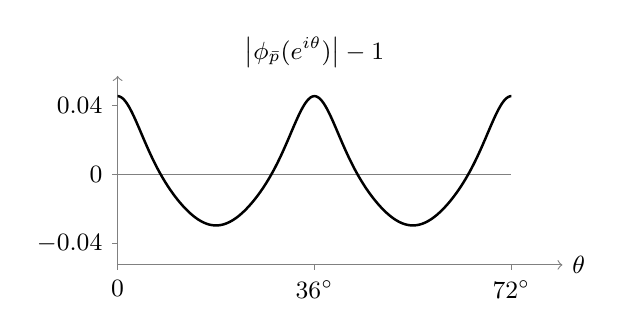
\begin{tikzpicture}[baseline=(current bounding box.center)]
  \draw[->, gray] (0,-1.15) -- (5.65,-1.15) node[right, black] {\small $\theta$};
  \draw[->, gray] (0,-1.15) -- (0,1.25);
  \draw[gray, line width=0.4pt] (0,0) -- (5.0,0);
  \foreach \x/\lab in {0/0, 2.5/{36^\circ}, 5.0/{72^\circ}} {
    \draw[gray] (\x,-1.15) -- (\x,-1.22) node[below, black] {\small $\lab$};
  }
  \foreach \y/\lab in {-0.88/{-0.04}, 0/0, 0.88/{0.04}} {
    \draw[gray] (0,\y) -- (-0.07,\y) node[left, black] {\small $\lab$};
  }
  \draw[line width=0.9pt] plot coordinates {(0.00000,0.99293) (0.00694,0.99260) (0.01389,0.99159) (0.02083,0.98991) (0.02778,0.98756) (0.03472,0.98456) (0.04167,0.98089) (0.04861,0.97658) (0.05556,0.97164) (0.06250,0.96606) (0.06944,0.95987) (0.07639,0.95307) (0.08333,0.94568) (0.09028,0.93772) (0.09722,0.92920) (0.10417,0.92014) (0.11111,0.91055) (0.11806,0.90045) (0.12500,0.88987) (0.13194,0.87882) (0.13889,0.86731) (0.14583,0.85538) (0.15278,0.84304) (0.15972,0.83032) (0.16667,0.81723) (0.17361,0.80379) (0.18056,0.79003) (0.18750,0.77596) (0.19444,0.76162) (0.20139,0.74701) (0.20833,0.73216) (0.21528,0.71710) (0.22222,0.70183) (0.22917,0.68638) (0.23611,0.67076) (0.24306,0.65501) (0.25000,0.63913) (0.25694,0.62314) (0.26389,0.60706) (0.27083,0.59090) (0.27778,0.57469) (0.28472,0.55843) (0.29167,0.54214) (0.29861,0.52584) (0.30556,0.50953) (0.31250,0.49324) (0.31944,0.47697) (0.32639,0.46073) (0.33333,0.44453) (0.34028,0.42839) (0.34722,0.41231) (0.35417,0.39631) (0.36111,0.38039) (0.36806,0.36455) (0.37500,0.34881) (0.38194,0.33317) (0.38889,0.31763) (0.39583,0.30221) (0.40278,0.28691) (0.40972,0.27173) (0.41667,0.25667) (0.42361,0.24175) (0.43056,0.22696) (0.43750,0.21230) (0.44444,0.19778) (0.45139,0.18340) (0.45833,0.16916) (0.46528,0.15507) (0.47222,0.14111) (0.47917,0.12731) (0.48611,0.11364) (0.49306,0.10012) (0.50000,0.08675) (0.50694,0.07352) (0.51389,0.06044) (0.52083,0.04750) (0.52778,0.03470) (0.53472,0.02205) (0.54167,0.00954) (0.54861,-0.00283) (0.55556,-0.01507) (0.56250,-0.02716) (0.56944,-0.03912) (0.57639,-0.05094) (0.58333,-0.06263) (0.59028,-0.07419) (0.59722,-0.08561) (0.60417,-0.09691) (0.61111,-0.10808) (0.61806,-0.11912) (0.62500,-0.13004) (0.63194,-0.14083) (0.63889,-0.15150) (0.64583,-0.16205) (0.65278,-0.17249) (0.65972,-0.18280) (0.66667,-0.19300) (0.67361,-0.20309) (0.68056,-0.21306) (0.68750,-0.22292) (0.69444,-0.23267) (0.70139,-0.24231) (0.70833,-0.25184) (0.71528,-0.26126) (0.72222,-0.27057) (0.72917,-0.27978) (0.73611,-0.28888) (0.74306,-0.29788) (0.75000,-0.30678) (0.75694,-0.31556) (0.76389,-0.32425) (0.77083,-0.33283) (0.77778,-0.34131) (0.78472,-0.34969) (0.79167,-0.35796) (0.79861,-0.36614) (0.80556,-0.37421) (0.81250,-0.38218) (0.81944,-0.39004) (0.82639,-0.39781) (0.83333,-0.40547) (0.84028,-0.41302) (0.84722,-0.42048) (0.85417,-0.42783) (0.86111,-0.43507) (0.86806,-0.44221) (0.87500,-0.44925) (0.88194,-0.45618) (0.88889,-0.46300) (0.89583,-0.46972) (0.90278,-0.47632) (0.90972,-0.48282) (0.91667,-0.48921) (0.92361,-0.49549) (0.93056,-0.50165) (0.93750,-0.50771) (0.94444,-0.51365) (0.95139,-0.51947) (0.95833,-0.52518) (0.96528,-0.53078) (0.97222,-0.53626) (0.97917,-0.54162) (0.98611,-0.54686) (0.99306,-0.55198) (1.00000,-0.55697) (1.00694,-0.56185) (1.01389,-0.56660) (1.02083,-0.57123) (1.02778,-0.57573) (1.03472,-0.58011) (1.04167,-0.58436) (1.04861,-0.58848) (1.05556,-0.59247) (1.06250,-0.59633) (1.06944,-0.60006) (1.07639,-0.60366) (1.08333,-0.60712) (1.09028,-0.61045) (1.09722,-0.61364) (1.10417,-0.61670) (1.11111,-0.61963) (1.11806,-0.62241) (1.12500,-0.62506) (1.13194,-0.62757) (1.13889,-0.62993) (1.14583,-0.63216) (1.15278,-0.63425) (1.15972,-0.63620) (1.16667,-0.63800) (1.17361,-0.63966) (1.18056,-0.64118) (1.18750,-0.64256) (1.19444,-0.64379) (1.20139,-0.64488) (1.20833,-0.64582) (1.21528,-0.64662) (1.22222,-0.64727) (1.22917,-0.64778) (1.23611,-0.64815) (1.24306,-0.64836) (1.25000,-0.64844) (1.25694,-0.64836) (1.26389,-0.64815) (1.27083,-0.64778) (1.27778,-0.64727) (1.28472,-0.64662) (1.29167,-0.64582) (1.29861,-0.64488) (1.30556,-0.64379) (1.31250,-0.64256) (1.31944,-0.64118) (1.32639,-0.63966) (1.33333,-0.63800) (1.34028,-0.63620) (1.34722,-0.63425) (1.35417,-0.63216) (1.36111,-0.62993) (1.36806,-0.62757) (1.37500,-0.62506) (1.38194,-0.62241) (1.38889,-0.61963) (1.39583,-0.61670) (1.40278,-0.61364) (1.40972,-0.61045) (1.41667,-0.60712) (1.42361,-0.60366) (1.43056,-0.60006) (1.43750,-0.59633) (1.44444,-0.59247) (1.45139,-0.58848) (1.45833,-0.58436) (1.46528,-0.58011) (1.47222,-0.57573) (1.47917,-0.57123) (1.48611,-0.56660) (1.49306,-0.56185) (1.50000,-0.55697) (1.50694,-0.55198) (1.51389,-0.54686) (1.52083,-0.54162) (1.52778,-0.53626) (1.53472,-0.53078) (1.54167,-0.52518) (1.54861,-0.51947) (1.55556,-0.51365) (1.56250,-0.50771) (1.56944,-0.50165) (1.57639,-0.49549) (1.58333,-0.48921) (1.59028,-0.48282) (1.59722,-0.47632) (1.60417,-0.46972) (1.61111,-0.46300) (1.61806,-0.45618) (1.62500,-0.44925) (1.63194,-0.44221) (1.63889,-0.43507) (1.64583,-0.42783) (1.65278,-0.42048) (1.65972,-0.41302) (1.66667,-0.40547) (1.67361,-0.39781) (1.68056,-0.39004) (1.68750,-0.38218) (1.69444,-0.37421) (1.70139,-0.36614) (1.70833,-0.35796) (1.71528,-0.34969) (1.72222,-0.34131) (1.72917,-0.33283) (1.73611,-0.32425) (1.74306,-0.31556) (1.75000,-0.30678) (1.75694,-0.29788) (1.76389,-0.28888) (1.77083,-0.27978) (1.77778,-0.27057) (1.78472,-0.26126) (1.79167,-0.25184) (1.79861,-0.24231) (1.80556,-0.23267) (1.81250,-0.22292) (1.81944,-0.21306) (1.82639,-0.20309) (1.83333,-0.19300) (1.84028,-0.18280) (1.84722,-0.17249) (1.85417,-0.16205) (1.86111,-0.15150) (1.86806,-0.14083) (1.87500,-0.13004) (1.88194,-0.11912) (1.88889,-0.10808) (1.89583,-0.09691) (1.90278,-0.08561) (1.90972,-0.07419) (1.91667,-0.06263) (1.92361,-0.05094) (1.93056,-0.03912) (1.93750,-0.02716) (1.94444,-0.01507) (1.95139,-0.00283) (1.95833,0.00954) (1.96528,0.02205) (1.97222,0.03470) (1.97917,0.04750) (1.98611,0.06044) (1.99306,0.07352) (2.00000,0.08675) (2.00694,0.10012) (2.01389,0.11364) (2.02083,0.12731) (2.02778,0.14111) (2.03472,0.15507) (2.04167,0.16916) (2.04861,0.18340) (2.05556,0.19778) (2.06250,0.21230) (2.06944,0.22696) (2.07639,0.24175) (2.08333,0.25667) (2.09028,0.27173) (2.09722,0.28691) (2.10417,0.30221) (2.11111,0.31763) (2.11806,0.33317) (2.12500,0.34881) (2.13194,0.36455) (2.13889,0.38039) (2.14583,0.39631) (2.15278,0.41231) (2.15972,0.42839) (2.16667,0.44453) (2.17361,0.46073) (2.18056,0.47697) (2.18750,0.49324) (2.19444,0.50953) (2.20139,0.52584) (2.20833,0.54214) (2.21528,0.55843) (2.22222,0.57469) (2.22917,0.59090) (2.23611,0.60706) (2.24306,0.62314) (2.25000,0.63913) (2.25694,0.65501) (2.26389,0.67076) (2.27083,0.68638) (2.27778,0.70183) (2.28472,0.71710) (2.29167,0.73216) (2.29861,0.74701) (2.30556,0.76162) (2.31250,0.77596) (2.31944,0.79003) (2.32639,0.80379) (2.33333,0.81723) (2.34028,0.83032) (2.34722,0.84304) (2.35417,0.85538) (2.36111,0.86731) (2.36806,0.87882) (2.37500,0.88987) (2.38194,0.90045) (2.38889,0.91055) (2.39583,0.92014) (2.40278,0.92920) (2.40972,0.93772) (2.41667,0.94568) (2.42361,0.95307) (2.43056,0.95987) (2.43750,0.96606) (2.44444,0.97164) (2.45139,0.97658) (2.45833,0.98089) (2.46528,0.98456) (2.47222,0.98756) (2.47917,0.98991) (2.48611,0.99159) (2.49306,0.99260) (2.50000,0.99293) (2.50694,0.99260) (2.51389,0.99159) (2.52083,0.98991) (2.52778,0.98756) (2.53472,0.98456) (2.54167,0.98089) (2.54861,0.97658) (2.55556,0.97164) (2.56250,0.96606) (2.56944,0.95987) (2.57639,0.95307) (2.58333,0.94568) (2.59028,0.93772) (2.59722,0.92920) (2.60417,0.92014) (2.61111,0.91055) (2.61806,0.90045) (2.62500,0.88987) (2.63194,0.87882) (2.63889,0.86731) (2.64583,0.85538) (2.65278,0.84304) (2.65972,0.83032) (2.66667,0.81723) (2.67361,0.80379) (2.68056,0.79003) (2.68750,0.77596) (2.69444,0.76162) (2.70139,0.74701) (2.70833,0.73216) (2.71528,0.71710) (2.72222,0.70183) (2.72917,0.68638) (2.73611,0.67076) (2.74306,0.65501) (2.75000,0.63913) (2.75694,0.62314) (2.76389,0.60706) (2.77083,0.59090) (2.77778,0.57469) (2.78472,0.55843) (2.79167,0.54214) (2.79861,0.52584) (2.80556,0.50953) (2.81250,0.49324) (2.81944,0.47697) (2.82639,0.46073) (2.83333,0.44453) (2.84028,0.42839) (2.84722,0.41231) (2.85417,0.39631) (2.86111,0.38039) (2.86806,0.36455) (2.87500,0.34881) (2.88194,0.33317) (2.88889,0.31763) (2.89583,0.30221) (2.90278,0.28691) (2.90972,0.27173) (2.91667,0.25667) (2.92361,0.24175) (2.93056,0.22696) (2.93750,0.21230) (2.94444,0.19778) (2.95139,0.18340) (2.95833,0.16916) (2.96528,0.15507) (2.97222,0.14111) (2.97917,0.12731) (2.98611,0.11364) (2.99306,0.10012) (3.00000,0.08675) (3.00694,0.07352) (3.01389,0.06044) (3.02083,0.04750) (3.02778,0.03470) (3.03472,0.02205) (3.04167,0.00954) (3.04861,-0.00283) (3.05556,-0.01507) (3.06250,-0.02716) (3.06944,-0.03912) (3.07639,-0.05094) (3.08333,-0.06263) (3.09028,-0.07419) (3.09722,-0.08561) (3.10417,-0.09691) (3.11111,-0.10808) (3.11806,-0.11912) (3.12500,-0.13004) (3.13194,-0.14083) (3.13889,-0.15150) (3.14583,-0.16205) (3.15278,-0.17249) (3.15972,-0.18280) (3.16667,-0.19300) (3.17361,-0.20309) (3.18056,-0.21306) (3.18750,-0.22292) (3.19444,-0.23267) (3.20139,-0.24231) (3.20833,-0.25184) (3.21528,-0.26126) (3.22222,-0.27057) (3.22917,-0.27978) (3.23611,-0.28888) (3.24306,-0.29788) (3.25000,-0.30678) (3.25694,-0.31556) (3.26389,-0.32425) (3.27083,-0.33283) (3.27778,-0.34131) (3.28472,-0.34969) (3.29167,-0.35796) (3.29861,-0.36614) (3.30556,-0.37421) (3.31250,-0.38218) (3.31944,-0.39004) (3.32639,-0.39781) (3.33333,-0.40547) (3.34028,-0.41302) (3.34722,-0.42048) (3.35417,-0.42783) (3.36111,-0.43507) (3.36806,-0.44221) (3.37500,-0.44925) (3.38194,-0.45618) (3.38889,-0.46300) (3.39583,-0.46972) (3.40278,-0.47632) (3.40972,-0.48282) (3.41667,-0.48921) (3.42361,-0.49549) (3.43056,-0.50165) (3.43750,-0.50771) (3.44444,-0.51365) (3.45139,-0.51947) (3.45833,-0.52518) (3.46528,-0.53078) (3.47222,-0.53626) (3.47917,-0.54162) (3.48611,-0.54686) (3.49306,-0.55198) (3.50000,-0.55697) (3.50694,-0.56185) (3.51389,-0.56660) (3.52083,-0.57123) (3.52778,-0.57573) (3.53472,-0.58011) (3.54167,-0.58436) (3.54861,-0.58848) (3.55556,-0.59247) (3.56250,-0.59633) (3.56944,-0.60006) (3.57639,-0.60366) (3.58333,-0.60712) (3.59028,-0.61045) (3.59722,-0.61364) (3.60417,-0.61670) (3.61111,-0.61963) (3.61806,-0.62241) (3.62500,-0.62506) (3.63194,-0.62757) (3.63889,-0.62993) (3.64583,-0.63216) (3.65278,-0.63425) (3.65972,-0.63620) (3.66667,-0.63800) (3.67361,-0.63966) (3.68056,-0.64118) (3.68750,-0.64256) (3.69444,-0.64379) (3.70139,-0.64488) (3.70833,-0.64582) (3.71528,-0.64662) (3.72222,-0.64727) (3.72917,-0.64778) (3.73611,-0.64815) (3.74306,-0.64836) (3.75000,-0.64844) (3.75694,-0.64836) (3.76389,-0.64815) (3.77083,-0.64778) (3.77778,-0.64727) (3.78472,-0.64662) (3.79167,-0.64582) (3.79861,-0.64488) (3.80556,-0.64379) (3.81250,-0.64256) (3.81944,-0.64118) (3.82639,-0.63966) (3.83333,-0.63800) (3.84028,-0.63620) (3.84722,-0.63425) (3.85417,-0.63216) (3.86111,-0.62993) (3.86806,-0.62757) (3.87500,-0.62506) (3.88194,-0.62241) (3.88889,-0.61963) (3.89583,-0.61670) (3.90278,-0.61364) (3.90972,-0.61045) (3.91667,-0.60712) (3.92361,-0.60366) (3.93056,-0.60006) (3.93750,-0.59633) (3.94444,-0.59247) (3.95139,-0.58848) (3.95833,-0.58436) (3.96528,-0.58011) (3.97222,-0.57573) (3.97917,-0.57123) (3.98611,-0.56660) (3.99306,-0.56185) (4.00000,-0.55697) (4.00694,-0.55198) (4.01389,-0.54686) (4.02083,-0.54162) (4.02778,-0.53626) (4.03472,-0.53078) (4.04167,-0.52518) (4.04861,-0.51947) (4.05556,-0.51365) (4.06250,-0.50771) (4.06944,-0.50165) (4.07639,-0.49549) (4.08333,-0.48921) (4.09028,-0.48282) (4.09722,-0.47632) (4.10417,-0.46972) (4.11111,-0.46300) (4.11806,-0.45618) (4.12500,-0.44925) (4.13194,-0.44221) (4.13889,-0.43507) (4.14583,-0.42783) (4.15278,-0.42048) (4.15972,-0.41302) (4.16667,-0.40547) (4.17361,-0.39781) (4.18056,-0.39004) (4.18750,-0.38218) (4.19444,-0.37421) (4.20139,-0.36614) (4.20833,-0.35796) (4.21528,-0.34969) (4.22222,-0.34131) (4.22917,-0.33283) (4.23611,-0.32425) (4.24306,-0.31556) (4.25000,-0.30678) (4.25694,-0.29788) (4.26389,-0.28888) (4.27083,-0.27978) (4.27778,-0.27057) (4.28472,-0.26126) (4.29167,-0.25184) (4.29861,-0.24231) (4.30556,-0.23267) (4.31250,-0.22292) (4.31944,-0.21306) (4.32639,-0.20309) (4.33333,-0.19300) (4.34028,-0.18280) (4.34722,-0.17249) (4.35417,-0.16205) (4.36111,-0.15150) (4.36806,-0.14083) (4.37500,-0.13004) (4.38194,-0.11912) (4.38889,-0.10808) (4.39583,-0.09691) (4.40278,-0.08561) (4.40972,-0.07419) (4.41667,-0.06263) (4.42361,-0.05094) (4.43056,-0.03912) (4.43750,-0.02716) (4.44444,-0.01507) (4.45139,-0.00283) (4.45833,0.00954) (4.46528,0.02205) (4.47222,0.03470) (4.47917,0.04750) (4.48611,0.06044) (4.49306,0.07352) (4.50000,0.08675) (4.50694,0.10012) (4.51389,0.11364) (4.52083,0.12731) (4.52778,0.14111) (4.53472,0.15507) (4.54167,0.16916) (4.54861,0.18340) (4.55556,0.19778) (4.56250,0.21230) (4.56944,0.22696) (4.57639,0.24175) (4.58333,0.25667) (4.59028,0.27173) (4.59722,0.28691) (4.60417,0.30221) (4.61111,0.31763) (4.61806,0.33317) (4.62500,0.34881) (4.63194,0.36455) (4.63889,0.38039) (4.64583,0.39631) (4.65278,0.41231) (4.65972,0.42839) (4.66667,0.44453) (4.67361,0.46073) (4.68056,0.47697) (4.68750,0.49324) (4.69444,0.50953) (4.70139,0.52584) (4.70833,0.54214) (4.71528,0.55843) (4.72222,0.57469) (4.72917,0.59090) (4.73611,0.60706) (4.74306,0.62314) (4.75000,0.63913) (4.75694,0.65501) (4.76389,0.67076) (4.77083,0.68638) (4.77778,0.70183) (4.78472,0.71710) (4.79167,0.73216) (4.79861,0.74701) (4.80556,0.76162) (4.81250,0.77596) (4.81944,0.79003) (4.82639,0.80379) (4.83333,0.81723) (4.84028,0.83032) (4.84722,0.84304) (4.85417,0.85538) (4.86111,0.86731) (4.86806,0.87882) (4.87500,0.88987) (4.88194,0.90045) (4.88889,0.91055) (4.89583,0.92014) (4.90278,0.92920) (4.90972,0.93772) (4.91667,0.94568) (4.92361,0.95307) (4.93056,0.95987) (4.93750,0.96606) (4.94444,0.97164) (4.95139,0.97658) (4.95833,0.98089) (4.96528,0.98456) (4.97222,0.98756) (4.97917,0.98991) (4.98611,0.99159) (4.99306,0.99260) (5.00000,0.99293)};
  \node at (2.5,1.55) {\small $\bigl|\phi_{\bar p}(e^{i\theta})\bigr|-1$};
\end{tikzpicture}

  \caption{The certified Schiffer shape.  Left: the image of the unit
  circle under $\phi_{\bar p}$ for the exact certificate center $\bar p$
  of \cite{ColbrookStepaniants2026,ColbrookStepaniantsCert2026} (solid),
  against the unit circle (dashed); the boundary radius varies between
  $0.9705$ and $1.0452$.  Right: the radial profile
  $\abs{\phi_{\bar p}(e^{i\theta})}-1$ over two of the ten symmetry
  periods.  Every domain $\Omega_\tau=\sqrt\tau\,\phi_{p_\tau}(\D)$ of
  \cref{thm:main} is a dilate of a small perturbation of this shape: the
  certified zero stays within $10^{-6}$ of $\bar x$ in the weighted norm.}
  \label{fig:domain}
\end{figure}

\begin{corollary}[Prescribed high contrast]\label{cor:contrast}
For every real $Q\ge1.03\times10^{16}$ there exists a bounded simply
connected non-disc with real-analytic Jordan boundary and constant relative
permittivity exactly $Q$ that is non-scattering for the same incident wave
\eqref{eq:herglotz} at exterior wavenumber one.
\end{corollary}

\subsection{Proof mechanism}

The argument has four steps.
\begin{enumerate}[leftmargin=2.2em]
  \item The Colbrook--Stepaniants theorem supplies a regular noncircular
  Schiffer zero in a weighted coefficient algebra.
  \item We introduce a Bessel-deformed fixed-disc equation $F_\tau=0$ whose
  zero is exactly equivalent to matching the physical Bessel Cauchy data.
  \item The implicit-function theorem gives a local branch abstractly, and
  explicit perturbation bounds show that the original contraction ball
  remains valid for all $0\le\tau\le10^{-13}$.
  \item Conformal covariance and dilation produce the physical domain,
  constant contrast, and exact zero scattered field.
\end{enumerate}
The full numerical provenance, the executable verifiers, and a Lean
re-verification of the certificate arithmetic are separated into the
accompanying verification supplement; the present article contains the
mathematical construction and proof.

\section{The certified Schiffer seed}\label{sec:seed}

We use the fixed-disc formulation of
\cite{ColbrookStepaniants2026}.  Let $X_\rho$ and $Y_\rho$ be their weighted
real coefficient spaces, with $\rho=1.05$.  A shape sequence has ten-fold
symmetry,
\begin{equation}\label{eq:p}
  p(z)=\sum_{j\ge0}p_jz^{10j},
  \qquad p_0>0,
\end{equation}
and is related to \eqref{eq:phi} by
\begin{equation}\label{eq:p-phi}
  p=p_0\phi_p'.
\end{equation}
The operator $K$ is an explicit inverse of the Laplacian on the compatible
coefficient range and satisfies
\begin{equation}\label{eq:K}
  \Delta K\gamma=\gamma,
  \qquad
  K\gamma=\partial_rK\gamma=0
  \quad\text{on }\partial\D.
\end{equation}
The Schiffer equation is
\begin{equation}\label{eq:F0}
  F_0(\gamma,p)
  :=\gamma+\abs{p}^2(1+K\gamma)=0.
\end{equation}
Indeed, if $W=K\gamma$ and $\widetilde u=1+W$, then
\[
  \Delta\widetilde u+\abs p^2\widetilde u=0
  \quad\text{in }\D,
  \qquad
  \widetilde u=1,
  \quad
  \partial_r\widetilde u=0
  \quad\text{on }\partial\D.
\]
Using \eqref{eq:p-phi}, the push-forward to $\phi_p(\D)$ has constant
interior squared wavenumber $p_0^2$.

The following summarizes precisely the consequences of the
Colbrook--Stepaniants computer-assisted theorem used here.

\begin{proposition}[Certified Schiffer seed]\label{prop:seed}
There is a center $\bar x=(\bar\gamma,\bar p)\in X_\rho$, a radius
$r=10^{-6}$, an invertible bounded operator
$\mathcal A:Y_\rho\to X_\rho$, and a unique exact zero
$x_\star=(\gamma_\star,p_\star)$ of $F_0$ in the closed ball
$B_r(\bar x)$ with the following properties.
\begin{enumerate}[label=\textup{(\alph*)},leftmargin=2.2em]
  \item Let $T_0=I-\mathcal AF_0$.  The certificate provides exact cubic
  Taylor majorants
  $Y\le1.59\times10^{-10}$, $Z\le0.621$, $C_2\le122$, $C_3\le0.012$ such
  that, on $B_r(\bar x)$,
  \[
    \sup_{B_r(\bar x)}\norm{T_0(x)-\bar x}\le Y+Zr+C_2r^2+C_3r^3,
    \qquad
    \sup_{B_r(\bar x)}\norm{DT_0}\le Z+2C_2r+3C_3r^2.
  \]
  Writing $R_0:=Y+Zr+C_2r^2+C_3r^3-r$ for the invariant-ball defect and
  $L_0:=Z+2C_2r+3C_3r^2$ for the contraction constant, exact rational
  evaluation gives
  \begin{align}
    R_0&\le-0.000000378718999999988<0,
    \label{eq:R0}\\
    L_0&\le0.621244000000036<1,
    \label{eq:L0}
  \end{align}
  so $T_0$ maps $B_r(\bar x)$ into itself and is a strict contraction
  there.
  \item Every $p$ in the ball satisfies
  \begin{equation}\label{eq:seedbounds}
    \norm p_\rho<55,
    \qquad 31<p_0<32,
    \qquad
    \sum_{j\ge1}\abs{p_j/p_0}<0.65.
  \end{equation}
  \item $\phi_p$ is univalent on a neighborhood of $\overline\D$, and its
  first nonconstant shape coefficient does not vanish.  Hence
  $\phi_p(\D)$ is a bounded simply connected non-disc with real-analytic
  Jordan boundary.
  \item The preconditioner satisfies
  \begin{equation}\label{eq:A}
    \norm{\mathcal A}<1180.
  \end{equation}
\end{enumerate}
\end{proposition}

\Cref{prop:seed} restates, in the notation of this paper, the certified
outputs of \cite[Eqs.~(3)--(5) and~(22), Lemma~2.4, Theorem~1.1]
{ColbrookStepaniants2026} and of the released validation certificate
\cite{ColbrookStepaniantsCert2026}, whose pinned hashes and replay commands
are recorded in the verification supplement.  The bound \eqref{eq:A}
follows from the upstream identity $C_3=\norm{\mathcal A}/(96\bar p_0^2)$
together with $C_3\le0.012$ and the exact center value $\bar p_0<32$:
\[
  \norm{\mathcal A}=96\bar p_0^2C_3<96\cdot32^2\cdot0.012=1179.648<1180.
\]
It therefore does not depend on reconstructing the norm of the upstream
approximate inverse to many digits.

\begin{remark}[Epistemic status]\label{rem:conditional}
\Cref{thm:main} is conditional on the computer-assisted theorem of
\cite{ColbrookStepaniants2026}, which at the time of writing is a very
recent preprint.  Everything imported from it is confined to
\cref{prop:seed}; the accompanying release pins the upstream certificate by
cryptographic hash, replays its authenticated checker, and machine-compares
every constant in \cref{prop:seed} against the pinned upstream data.
\end{remark}

\begin{lemma}[Regularity of the certified zero]\label{lem:regular}
The derivative $DF_0(x_\star):X_\rho\to Y_\rho$ is a bounded linear
isomorphism.
\end{lemma}

\begin{proof}
At the fixed point,
\[
  DT_0(x_\star)=I-\mathcal ADF_0(x_\star).
\]
By \eqref{eq:L0}, $\norm{DT_0(x_\star)}<1$.  Hence
$I-DT_0(x_\star)=\mathcal ADF_0(x_\star)$ is invertible by the
Neumann-series lemma.  Since $\mathcal A$ is invertible, so is
$DF_0(x_\star)$.
\end{proof}

\section{The Bessel-deformed transmission equation}\label{sec:deformation}

For $\tau\ge0$, define
\begin{equation}\label{eq:H}
  H_{\tau,p}(z)
  :=\sum_{n=0}^{\infty}
  \frac{(-1)^n}{(n!)^2}
  \left(\frac{\tau\abs{\phi_p(z)}^2}{4}\right)^n.
\end{equation}
For $\tau>0$,
\begin{equation}\label{eq:HJ0}
  H_{\tau,p}(z)=J_0\!\left(\sqrt\tau\,\abs{\phi_p(z)}\right),
\end{equation}
and $H_{0,p}=1$.  The power-series definition makes the dependence on
$\tau$ analytic at zero.  Conformal covariance of the Laplacian and
\eqref{eq:p-phi} give
\begin{equation}\label{eq:Hpde}
  \Delta H_{\tau,p}
  +\frac{\tau}{p_0^2}\abs p^2H_{\tau,p}=0
  \quad\text{in }\D.
\end{equation}

We now define the deformed operator
\begin{equation}\label{eq:Ftau}
  F_\tau(\gamma,p)
  :=\gamma+\abs p^2K\gamma
   +\abs p^2\left(1-\frac\tau{p_0^2}\right)H_{\tau,p}.
\end{equation}
At $\tau=0$, this is exactly \eqref{eq:F0}.

\begin{lemma}[Fixed-disc transmission identity]\label{lem:fixed-disc}
If $F_\tau(\gamma,p)=0$ and
\begin{equation}\label{eq:Utilde}
  \widetilde U_{\tau,p}:=H_{\tau,p}+K\gamma,
\end{equation}
then
\begin{equation}\label{eq:Utildepde}
  \Delta\widetilde U_{\tau,p}
  +\abs p^2\widetilde U_{\tau,p}=0
  \quad\text{in }\D.
\end{equation}
Moreover, $\widetilde U_{\tau,p}$ and $H_{\tau,p}$ have identical
Dirichlet and radial Neumann traces on $\partial\D$.
\end{lemma}

\begin{proof}
Using \eqref{eq:K} and \eqref{eq:Hpde}, the left-hand side of
\eqref{eq:Utildepde} is exactly $F_\tau(\gamma,p)$.  The trace statement
follows from the two clamped trace identities in \eqref{eq:K}.
\end{proof}

The preceding equation reveals the continuation mechanism independently of
the particular numerical seed.

\begin{theorem}[Regular Schiffer zeros generate physical non-scatterers]
\label{thm:abstract}
Let $x_\star=(\gamma_\star,p_\star)$ be a zero of $F_0$ such that
$DF_0(x_\star)$ is invertible, $p_{\star,0}>0$, and $\phi_{p_\star}$ is
univalent on a neighborhood of $\overline\D$ and non-affine.  Then there
are $\varepsilon>0$ and a real-analytic branch
\[
  (-\varepsilon,\varepsilon)\ni\tau
  \longmapsto x_\tau=(\gamma_\tau,p_\tau)
\]
with $F_\tau(x_\tau)=0$ and $x_\tau\to x_\star$ as $\tau\to0$.  For every
sufficiently small $\tau>0$, the scaled domain
$\sqrt\tau\,\phi_{p_\tau}(\D)$ is a noncircular homogeneous dielectric that
is exactly non-scattering for the incident wave \eqref{eq:herglotz} at
exterior wavenumber one.
\end{theorem}

\begin{proof}
The series \eqref{eq:H} converges normally in a neighborhood of
$(0,x_\star)$ in the weighted coefficient algebra.  Hence
$(\tau,x)\mapsto F_\tau(x)$ is real analytic there.  The analytic
implicit-function theorem and the invertibility of $DF_0(x_\star)$ produce
the branch.  Univalence on a complex collar and non-affineness are open in
the weighted coefficient norm, so they persist for small $\tau$.
Non-affineness excludes a disc through the ten-fold symmetry of the ansatz
\eqref{eq:phi}: with $\omega=e^{2\pi i/10}$ one has
$\phi_p(\omega z)=\omega\phi_p(z)$, so the image is invariant under
rotation by $\omega$; a disc with this invariance is centered at the
origin, and the unique Riemann map of $\D$ onto such a disc with
$\phi(0)=0$ and $\phi'(0)>0$ is linear.  A non-affine $\phi_p$ therefore
cannot map $\D$ onto a disc.

For $\tau>0$, \cref{lem:fixed-disc} supplies two fields with equal Cauchy
data on the unit circle.  Pushing them forward by $\phi_{p_\tau}$ gives
exterior squared wavenumber $\tau$ and interior squared wavenumber
$p_{\tau,0}^2$.  Dilation by $\sqrt\tau$ fixes the exterior wavenumber at
one and changes the interior squared wavenumber to
$p_{\tau,0}^2/\tau$.  The complete physical verification is given in
\cref{sec:physical}.
\end{proof}

\section{A uniform certified branch}\label{sec:quantitative}

The abstract theorem gives a local branch but no explicit interval.  We now
show that the entire Schiffer contraction ball remains valid for
$0\le\tau\le10^{-13}$.  Put
\[
  \delta F_\tau:=F_\tau-F_0.
\]
All norms below are the weighted coefficient majorants of
\cite{ColbrookStepaniants2026}.  One structural property of that algebra is
used repeatedly and deserves to be isolated.

\begin{lemma}[Radial multiplication is nonexpansive]\label{lem:radial}
In the weighted coefficient algebra of
\cite{ColbrookStepaniants2026,ColbrookStepaniantsCert2026} the norm is a
weighted $\ell^1$ sum over a basis indexed by an angular block index $\ell$
and a radial index $s$, with weight $c_\ell\rho^\ell$ depending on $\ell$
only.  Multiplication by the radial factor $\abs z^2$ raises the radial
index and leaves the angular index and the weight unchanged.  Hence
$\norm{\abs z^2f}\le\norm f$ for every $f$, and for any product
decomposition $\phi_p(z)=z\psi_p(z)$,
\[
  \norm{\abs{\phi_p}^2}
  =\norm{\abs z^2\abs{\psi_p}^2}
  \le\norm{\psi_p}^2 .
\]
\end{lemma}

\begin{proof}
The norm and the multiplication recurrences are specified in
\cite[Validation Specification, \S\S2 and~4]{ColbrookStepaniantsCert2026}:
the weights are $c_\ell\rho^\ell$ with $c_0=1$, $c_\ell=2$, independent of
the radial index, and multiplication by $r^2$ acts as the pure radial shift
$(\ell,s)\mapsto(\ell,s+1)$.  A shift with unchanged weights does not
increase a weighted $\ell^1$ norm, and the final inequality is
submultiplicativity of the algebra norm.
\end{proof}

Write $\phi_p(z)=z\psi_p(z)$.  From \eqref{eq:phi} and
\eqref{eq:seedbounds},
\begin{equation}\label{eq:psi}
  \norm{\psi_p}
  \le1+\frac1{11p_0}\sum_{j\ge1}\abs{p_j}\rho^j
  \le1+\frac{\norm p_\rho-p_0}{11\cdot31}
  \le1+\frac{55-31}{11\cdot31}
  <\frac{11}{10},
\end{equation}
and therefore, by \cref{lem:radial},
\begin{equation}\label{eq:phisq}
  \norm{\abs{\phi_p}^2}\le\norm{\psi_p}^2<\frac{121}{100}<\frac54.
\end{equation}
Set $u=\tau\norm{\abs{\phi_p}^2}/4$.  For
$0\le\tau\le10^{-13}$, $u<1/2$.  The full series \eqref{eq:H}, without
truncation, therefore gives
\begin{equation}\label{eq:Hbounds}
  \norm{H_{\tau,p}}\le2,
  \qquad
  \norm{H_{\tau,p}-1}\le\frac58\tau.
\end{equation}
Since $p_0>31$,
\begin{align}
 \norm{\left(1-\frac\tau{p_0^2}\right)H_{\tau,p}-1}
 &\le \norm{H_{\tau,p}-1}
      +\frac\tau{p_0^2}\norm{H_{\tau,p}}\notag\\
 &<\frac{63}{100}\tau.
 \label{eq:Bbound}
\end{align}
Multiplication by $\norm p^2<55^2$ yields
\begin{equation}\label{eq:value}
  \boxed{\norm{\delta F_\tau}<1906\tau.}
\end{equation}

For the derivative estimate, let $\xi$ be a shape variation of full
$X_\rho$ norm at most one.  The upstream product norm weights the shape
block by $2\bar p_0\rho^j$
\cite[Validation Specification, Eq.~(13)]{ColbrookStepaniantsCert2026},
so
\begin{equation}\label{eq:xibounds}
  \norm\xi\le\frac1{2\bar p_0}<\frac1{62},
  \qquad
  \abs{\xi_0}<\frac1{62}.
\end{equation}
Differentiating \eqref{eq:phi} and using \eqref{eq:seedbounds} gives
\begin{equation}\label{eq:Dpsi}
  \norm{D\psi_p[\xi]}
  \le\frac1{11}
  \left(\frac{\norm\xi}{31}
  +\frac{55\abs{\xi_0}}{31^2}\right)
  <\frac1{7000}.
\end{equation}
Consequently
\begin{equation}\label{eq:DRDH}
  \norm{D\abs{\phi_p}^2[\xi]}
  \le2\norm{\psi_p}\norm{D\psi_p[\xi]}
  <\frac1{3000},
  \qquad
  \norm{DH_{\tau,p}[\xi]}\le\frac\tau{3000},
\end{equation}
where the first estimate again uses \cref{lem:radial}.
Differentiating \eqref{eq:Ftau}, and combining
\eqref{eq:Bbound}, \eqref{eq:Hbounds}, \eqref{eq:xibounds}, and
\eqref{eq:DRDH}, gives
\begin{equation}\label{eq:derivative}
  \boxed{\norm{D\delta F_\tau}<3\tau.}
\end{equation}
The elementary constant arithmetic behind \eqref{eq:value} and
\eqref{eq:derivative} is recorded in the verification supplement.

Define
\[
  T_\tau(x)=x-\mathcal AF_\tau(x).
\]
On the original radius-$r$ ball,
\eqref{eq:A}, \eqref{eq:value}, and \eqref{eq:derivative} give
\begin{align}
  R_\tau&\le R_0+1180\cdot1906\,\tau,
  \label{eq:Rtau}\\
  L_\tau&\le L_0+1180\cdot3\,\tau.
  \label{eq:Ltau}
\end{align}
At $\tau_*=10^{-13}$,
\begin{align}
  R_{\tau_*}
  &\le-0.000000153810999999988<0,
  \label{eq:Rend}\\
  L_{\tau_*}
  &\le0.621244000354036<1.
  \label{eq:Lend}
\end{align}
The right-hand sides of \eqref{eq:Rtau}--\eqref{eq:Ltau} increase with
$\tau$.  Hence $T_\tau$ maps the same closed ball into itself and is a
strict contraction for every $0\le\tau\le\tau_*$.  Banach's theorem gives a
unique exact zero
\begin{equation}\label{eq:branch}
  x_\tau=(\gamma_\tau,p_\tau)\in B_r(\bar x)
  \qquad(0\le\tau\le10^{-13}).
\end{equation}
Because the whole branch stays in the certified ball, all univalence,
analytic-boundary, and noncircularity conclusions of
\cref{prop:seed} hold uniformly.

\section{The physical inclusion and exact zero scattering}\label{sec:physical}

Fix $0<\tau\le10^{-13}$ and the exact zero
$x_\tau=(\gamma_\tau,p_\tau)$ from \eqref{eq:branch}.  Define the domain and
contrast by \eqref{eq:Omegaq}.  For $y\in\Omega_\tau$, put
\[
  z=\phi_{p_\tau}^{-1}\!\left(\frac y{\sqrt\tau}\right)
\]
and define
\begin{equation}\label{eq:U}
  U_\tau(y)
  =\sqrt{2\pi}\left[
    H_{\tau,p_\tau}(z)+K\gamma_\tau(z)
  \right].
\end{equation}
Since $y=\sqrt\tau\,\phi_{p_\tau}(z)$,
\begin{equation}\label{eq:HtoJ}
  H_{\tau,p_\tau}(z)=J_0(\abs y).
\end{equation}

Conformal covariance transforms \eqref{eq:Utildepde} into an interior
Helmholtz equation with squared wavenumber $p_{\tau,0}^2$ on
$\phi_{p_\tau}(\D)$.  The dilation $y=\sqrt\tau\,x$ therefore gives
\begin{equation}\label{eq:Upde}
  (\Delta_y+q_\tau)U_\tau=0
  \quad\text{in }\Omega_\tau,
  \qquad
  q_\tau=\frac{p_{\tau,0}^2}{\tau}.
\end{equation}
By \eqref{eq:seedbounds},
\begin{equation}\label{eq:qnot1}
  q_\tau>\frac{31^2}{10^{-13}}>1,
\end{equation}
so $q_\tau$ is positive and nonunit.

It remains to check the traces.  The difference between the pulled-back
interior field and the pulled-back incident field is $K\gamma_\tau$, whose
Dirichlet and radial Neumann traces vanish by \eqref{eq:K}.  Under a
conformal map the normal derivative is multiplied by a nonzero boundary
scale factor, and under dilation it is multiplied by another nonzero
constant.  Thus zero remains zero, and \eqref{eq:HtoJ} gives
\begin{equation}\label{eq:physicaltraces}
  U_\tau=v,
  \qquad
  \partial_\nu U_\tau=\partial_\nu v
  \quad\text{on }\partial\Omega_\tau.
\end{equation}

For completeness, writing $d=(\cos\theta,\sin\theta)$,
\[
  \int_0^{2\pi}e^{ix\cdot d}\dd\theta
  =2\pi J_0(\abs x),
\]
so \eqref{eq:herglotz} follows, and
\[
  \norm h_{L^2(\Sone)}^2
  =\int_0^{2\pi}\frac1{2\pi}\dd\theta=1.
\]
The incident field is therefore a nonzero normalized $L^2$-Herglotz wave.

Define the total field piecewise by $U_\tau$ in $\Omega_\tau$ and by $v$ in
the exterior.  Equation \eqref{eq:physicaltraces} makes it a transmission
solution.  Its exterior scattered component is identically zero, which
satisfies the Sommerfeld radiation condition and has zero far-field pattern.
Because $q_\tau$ is a bounded positive constant, the direct transmission
problem for the incident field $v$ has exactly one solution
\cite[Chapter~8]{ColtonKress2019}; the solution just exhibited is therefore
the physical total field, and the scattered field of $\Omega_\tau$ for $v$
vanishes identically.  This proves \cref{thm:main}.

\section{Consequences and interpretation}\label{sec:consequences}

\subsection{Prescribing the contrast}

The contraction maps $T_\tau$ depend continuously on $\tau$ and have a
uniform Lipschitz constant strictly below one.  Hence their unique fixed
points depend continuously on $\tau$.  One may see this directly from
\begin{equation}\label{eq:stability}
  \norm{x_\tau-x_\sigma}
  \le
  \frac{\norm{T_\tau(x_\sigma)-T_\sigma(x_\sigma)}}{1-L},
\end{equation}
where $L<1$ is any common contraction constant.  Thus
$\tau\mapsto p_{\tau,0}$ and
\[
  q_\tau=\frac{p_{\tau,0}^2}{\tau}
\]
are continuous on $(0,10^{-13}]$.  Since
$p_{\tau,0}\to p_{\star,0}>31$ as $\tau\downarrow0$,
\begin{equation}\label{eq:qinfty}
  q_\tau\longrightarrow+\infty.
\end{equation}
At $\tau_*=10^{-13}$, the upper bound $p_{\tau_*,0}<32$ gives
\begin{equation}\label{eq:qendpoint}
  q_{\tau_*}
  <\frac{32^2}{10^{-13}}
  =1.024\times10^{16}.
\end{equation}
For any $Q\ge1.03\times10^{16}$, choose $\delta>0$ small enough that
$q_\delta>Q$.  The intermediate-value theorem on
$[\delta,\tau_*]$ and \eqref{eq:qendpoint} produce some $\tau$ with
$q_\tau=Q$.  This proves \cref{cor:contrast}.

\subsection{The subwavelength/high-index regime}

At fixed exterior wavenumber one, the diameter of $\Omega_\tau$ is
$O(\sqrt\tau)$, whereas
\begin{equation}\label{eq:opticalsize}
  \sqrt{q_\tau}\,\sqrt\tau=p_{\tau,0}
  \longrightarrow p_{\star,0}\approx31.967.
\end{equation}
Thus the family maintains a finite interior optical size by increasing the
positive refractive index as the physical inclusion shrinks.  The result is
an existence theorem for homogeneous, passive, positive-index material, but
it does not yet reach moderate contrast.  Natural next questions are whether
other Schiffer branches, nonradial Herglotz controls, or continuation farther
from $\tau=0$ can reduce the required contrast, and whether an analogous
mechanism exists for the full three-dimensional vector Maxwell system.

\section*{Reproducibility and formal verification}

The accompanying release contains the exact certificate data, independent
exact-arithmetic verifiers that rederive the perturbation constants of
\cref{sec:quantitative} from the certified ball bounds, the pinned and
replayed upstream dependency, and a Lean~4 re-verification of the exact
rational certificate arithmetic together with generic fixed-point lemmas in
the form used here.  The Lean development does not formalize the operator
estimates, the upstream certificate, or the scattering analysis; its exact
boundary, the numerical provenance, and the replay commands are recorded in
a separate verification supplement so that they do not obscure the
mathematical argument above.

\section*{Declaration of computational assistance}

The author gratefully acknowledges \textbf{GPT-5.6 Sol Pro} (OpenAI), which
was used extensively as a research and development assistant for theorem
exploration, literature synthesis, symbolic and numerical checking, code and
Lean-formalization generation, and drafting and editing this manuscript.  The
author reviewed and revised all generated material and takes responsibility
for every mathematical claim, computation, and conclusion in the submitted
work.

\begin{thebibliography}{CCH16}

\bibitem[Ber80]{Berenstein1980}
Carlos A. Berenstein.
\newblock An inverse spectral theorem and its relation to the {Pompeiu} problem.
\newblock \emph{J. Analyse Math.} 37 (1980), 128--144.

\bibitem[BPS14]{BlastenPaivarintaSylvester2014}
Eemeli Bl{\aa}sten, Lassi P{\"a}iv{\"a}rinta, and John Sylvester.
\newblock Corners always scatter.
\newblock \emph{Comm. Math. Phys.} 331 (2014), no.~2, 725--753.

\bibitem[BST73]{BrownSchreiberTaylor1973}
Leon Brown, Bertram M. Schreiber, and B. Alan Taylor.
\newblock Spectral synthesis and the {Pompeiu} problem.
\newblock \emph{Ann. Inst. Fourier (Grenoble)} 23 (1973), no.~3, 125--154.

\bibitem[CCH16]{CakoniColtonHaddar2016}
Fioralba Cakoni, David Colton, and Houssem Haddar.
\newblock \emph{Inverse Scattering Theory and Transmission Eigenvalues}.
\newblock CBMS-NSF Regional Conference Series in Applied Mathematics 88, SIAM,
Philadelphia, 2016.

\bibitem[CV23]{CakoniVogelius2023}
Fioralba Cakoni and Michael S. Vogelius.
\newblock Singularities almost always scatter: regularity results for
non-scattering inhomogeneities.
\newblock \emph{Comm. Pure Appl. Math.} 76 (2023), no.~12, 4022--4047.

\bibitem[CV26]{CakoniVogelius2026}
Fioralba Cakoni and Michael S. Vogelius.
\newblock Transmission eigenvalues and non-scattering.
\newblock arXiv:2602.06250, 2026.

\bibitem[CVX23]{CakoniVogeliusXiao2023}
Fioralba Cakoni, Michael S. Vogelius, and Jingni Xiao.
\newblock On the regularity of non-scattering anisotropic inhomogeneities.
\newblock \emph{Arch. Ration. Mech. Anal.} (2023), doi:10.1007/s00205-023-01863-y.

\bibitem[CDP26]{CaoLaboraDeDiosPont2026}
Gonzalo Cao-Labora and Jaume de Dios Pont.
\newblock Counterexamples to {Schiffer}'s conjecture.
\newblock arXiv:2608.05114, 2026.

\bibitem[CS26]{ColbrookStepaniants2026}
Matthew J. Colbrook and George Stepaniants.
\newblock A computer-assisted counterexample to the planar {Pompeiu} and
{Schiffer} conjectures.
\newblock arXiv:2608.01579, 2026.

\bibitem[CS26c]{ColbrookStepaniantsCert2026}
Matthew J. Colbrook and George Stepaniants.
\newblock {Pompeiu}--{Schiffer} validation certificate v1.0.0.
\newblock Zenodo, 2026, doi:10.5281/zenodo.21765287.

\bibitem[CK19]{ColtonKress2019}
David Colton and Rainer Kress.
\newblock \emph{Inverse Acoustic and Electromagnetic Scattering Theory}.
\newblock 4th edition, Applied Mathematical Sciences 93, Springer, Cham, 2019.

\bibitem[CM88]{ColtonMonk1988}
David Colton and Peter Monk.
\newblock The inverse scattering problem for time-harmonic acoustic waves in
an inhomogeneous medium.
\newblock \emph{Quart. J. Mech. Appl. Math.} 41 (1988), no.~1, 97--125.

\bibitem[EH15]{ElschnerHu2015}
Johannes Elschner and Guanghui Hu.
\newblock Corners and edges always scatter.
\newblock \emph{Inverse Problems} 31 (2015), no.~1, 015003.

\bibitem[HV25]{HovsepyanVogelius2025}
Narek Hovsepyan and Michael S. Vogelius.
\newblock Scattering from analytic and piecewise analytic inhomogeneities.
\newblock arXiv:2507.13986, 2025.

\bibitem[Kir86]{Kirsch1986}
Andreas Kirsch.
\newblock The denseness of the far field patterns for the transmission problem.
\newblock \emph{IMA J. Appl. Math.} 37 (1986), no.~3, 213--225.

\bibitem[PSV17]{PaivarintaSaloVesalainen2017}
Lassi P{\"a}iv{\"a}rinta, Mikko Salo, and Esa V. Vesalainen.
\newblock Strictly convex corners scatter.
\newblock \emph{Rev. Mat. Iberoam.} 33 (2017), no.~4, 1369--1396.

\bibitem[Pom29]{Pompeiu1929}
Dimitrie Pompeiu.
\newblock Sur certains syst\`emes d'\'equations lin\'eaires et sur une
propri\'et\'e int\'egrale des fonctions de plusieurs variables.
\newblock \emph{C. R. Acad. Sci. Paris} 188 (1929), 1138--1139.

\bibitem[SS21]{SaloShahgholian2021}
Mikko Salo and Henrik Shahgholian.
\newblock Free boundary methods and non-scattering phenomena.
\newblock \emph{Res. Math. Sci.} 8 (2021), no.~4, Paper No. 58.

\bibitem[VX21]{VogeliusXiao2021}
Michael S. Vogelius and Jingni Xiao.
\newblock Finiteness results concerning nonscattering wave numbers for
incident plane and {Herglotz} waves.
\newblock \emph{SIAM J. Math. Anal.} 53 (2021), no.~5, doi:10.1137/20M1367854.

\bibitem[Wil76]{Williams1976}
Stephen A. Williams.
\newblock A partial solution of the {Pompeiu} problem.
\newblock \emph{Math. Ann.} 223 (1976), no.~2, 183--190.

\end{thebibliography}


\end{document}
